\documentclass[twoside]{book}

% Packages required by doxygen
\usepackage{calc}
\usepackage{doxygen}
\usepackage{graphicx}
\usepackage[utf8]{inputenc}
\usepackage{makeidx}
\usepackage{multicol}
\usepackage{multirow}
\usepackage{textcomp}
\usepackage[table]{xcolor}

% NLS support packages
\usepackage{polski}
\usepackage[T1]{fontenc}

% Font selection
\usepackage[T1]{fontenc}
\usepackage{mathptmx}
\usepackage[scaled=.90]{helvet}
\usepackage{courier}
\usepackage{amssymb}
\usepackage{sectsty}
\renewcommand{\familydefault}{\sfdefault}
\allsectionsfont{%
  \fontseries{bc}\selectfont%
  \color{darkgray}%
}
\renewcommand{\DoxyLabelFont}{%
  \fontseries{bc}\selectfont%
  \color{darkgray}%
}

% Page & text layout
\usepackage{geometry}
\geometry{%
  a4paper,%
  top=2.5cm,%
  bottom=2.5cm,%
  left=2.5cm,%
  right=2.5cm%
}
\tolerance=750
\hfuzz=15pt
\hbadness=750
\setlength{\emergencystretch}{15pt}
\setlength{\parindent}{0cm}
\setlength{\parskip}{0.2cm}
\makeatletter
\renewcommand{\paragraph}{%
  \@startsection{paragraph}{4}{0ex}{-1.0ex}{1.0ex}{%
    \normalfont\normalsize\bfseries\SS@parafont%
  }%
}
\renewcommand{\subparagraph}{%
  \@startsection{subparagraph}{5}{0ex}{-1.0ex}{1.0ex}{%
    \normalfont\normalsize\bfseries\SS@subparafont%
  }%
}
\makeatother

% Headers & footers
\usepackage{fancyhdr}
\pagestyle{fancyplain}
\fancyhead[LE]{\fancyplain{}{\bfseries\thepage}}
\fancyhead[CE]{\fancyplain{}{}}
\fancyhead[RE]{\fancyplain{}{\bfseries\leftmark}}
\fancyhead[LO]{\fancyplain{}{\bfseries\rightmark}}
\fancyhead[CO]{\fancyplain{}{}}
\fancyhead[RO]{\fancyplain{}{\bfseries\thepage}}
\fancyfoot[LE]{\fancyplain{}{}}
\fancyfoot[CE]{\fancyplain{}{}}
\fancyfoot[RE]{\fancyplain{}{\bfseries\scriptsize Wygenerowano Pt, 24 cze 2016 18\-:45\-:10 dla Średniowiecze programem Doxygen }}
\fancyfoot[LO]{\fancyplain{}{\bfseries\scriptsize Wygenerowano Pt, 24 cze 2016 18\-:45\-:10 dla Średniowiecze programem Doxygen }}
\fancyfoot[CO]{\fancyplain{}{}}
\fancyfoot[RO]{\fancyplain{}{}}
\renewcommand{\footrulewidth}{0.4pt}
\renewcommand{\chaptermark}[1]{%
  \markboth{#1}{}%
}
\renewcommand{\sectionmark}[1]{%
  \markright{\thesection\ #1}%
}

% Indices & bibliography
\usepackage{natbib}
\usepackage[titles]{tocloft}
\setcounter{tocdepth}{3}
\setcounter{secnumdepth}{5}
\makeindex

% Hyperlinks (required, but should be loaded last)
\usepackage{ifpdf}
\ifpdf
  \usepackage[pdftex,pagebackref=true]{hyperref}
\else
  \usepackage[ps2pdf,pagebackref=true]{hyperref}
\fi
\hypersetup{%
  colorlinks=true,%
  linkcolor=blue,%
  citecolor=blue,%
  unicode%
}

% Custom commands
\newcommand{\clearemptydoublepage}{%
  \newpage{\pagestyle{empty}\cleardoublepage}%
}


%===== C O N T E N T S =====

\begin{document}

% Titlepage & ToC
\hypersetup{pageanchor=false}
\pagenumbering{roman}
\begin{titlepage}
\vspace*{7cm}
\begin{center}%
{\Large Średniowiecze }\\
\vspace*{1cm}
{\large Wygenerowano przez Doxygen 1.8.6}\\
\vspace*{0.5cm}
{\small Pt, 24 cze 2016 18:45:10}\\
\end{center}
\end{titlepage}
\clearemptydoublepage
\tableofcontents
\clearemptydoublepage
\pagenumbering{arabic}
\hypersetup{pageanchor=true}

%--- Begin generated contents ---
\chapter{Dokumentacja Zadania Średniowiecze}
\label{index}\hypertarget{index}{}\section*{Średniowiecze}

Uwaga\-: aktualna treść zadania znajduje się w \href{https://moodle.mimuw.edu.pl/mod/assignment/view.php?id=18178}{\tt Moodle'u}.

\subsubsection*{Opis projektu}

Dużym, trzyczęściowym projektem zaliczeniowym w tym roku jest implementacja deterministycznej turowej gry strategicznej z pełną wiedzą wraz ze sztuczną inteligencją (A\-I). Pierwsza część polega na zaimplementowaniu i przetestowaniu struktur danych oraz protokołu wejścia w programie A\-I. W drugiej części należy stworzyć nic nie robiącą A\-I oraz skrypt bash łączący program interfejsu graficznego i programy A\-I w symulator rozgrywki A\-I vs A\-I, A\-I vs człowiek lub człowiek vs człowiek. W trzeciej i ostatniej części należy stworzyć A\-I potrafiące wygrać przeciwko prostym strategiom.

\subsubsection*{Opis gry}

Gra rozgrywa się na kwadratowej planszy {\ttfamily n$\ast$n} ({\ttfamily 8 $<$ n $<$ 2$^\wedge$31}) i jest przeznaczona dla dwóch graczy wykonujących na zmianę swoje tury (rozpoczynając od pierwszego gracza). Każdy z graczy kontroluje swoje jednostki należące do jednego z trzech typów\-: król, rycerz, chłop. Na początku gry każdy gracz ma 1 króla, 1 chłopa i 2 rycerzy, ustawionych jeden obok drugiego w poziomej linii na planszy w kolejności król, chłop, rycerz, rycerz. Początkowe ustawienie jednostek następuje poprzez wylosowanie pozycji królów spośród pierwszych {\ttfamily n-\/3} kolumn, tak aby królowie byli od siebie oddaleni o co najmniej 8 w metryce maksimum.

Podczas każdej tury gracz może ruszyć raz każdą swoją jednostką. Ruch składa się z przesunięcia jej o 1 pole pionowo, poziomo, na skos lub wykonania akcji (tylko przez chłopa). Gdy jednostka ruszy się na pole zajmowane przez inną jednostkę, następuje walka. Gdy walczą ze sobą dwie jednostki tego samego typu, obie giną. W przeciwnym wypadku rycerz pokonuje króla lub chłopa, a król pokonuje chłopa. Nie można ruszyć swojej jednostki na pole zajmowane przez inną swoją jednostkę (aczkolwiek można najpierw przesunąć jedną jednostkę, a drugą później przesunąć na zwolnione miejsce w tej samej turze). Akcją możliwą do wykonania przez chłopa jest wyprodukowanie nowego rycerza albo chłopa na jednym z sąsiednich (pionowo, poziomo lub po skosie) wolnych pól, pod warunkiem że chłop stał w miejscu, nie wykonując akcji przez poprzednie 2 tury. Innymi słowy chłop, który ruszył się w turze {\ttfamily k}, a potem się już nie ruszał, może dopiero wyprodukować jednostkę w turze {\ttfamily k+3}, następnie {\ttfamily k+6} itd. Nowymi jednostkami można się ruszać od razu po wyprodukowaniu (tj. gdy zostały wyprodukowane w turze {\ttfamily k}, to traktowane są jakby ostatnio wykonały ruch w turze {\ttfamily k-\/1}). Chłop, który od początku gry (tura 1) się nie ruszał, może wyprodukować pierwszą jednostkę w turze 3, a każda jednostka na początku gry może się od razu ruszyć.

Gra kończy się w momencie, gdy król jednego z graczy zginie lub po {\ttfamily k}-\/tej ({\ttfamily 1 $<$= k $<$ 2$^\wedge$31}) turze drugiego gracza. Wygrywa gracz mający jedynego żywego króla. W przeciwnym wypadku mamy remis.

\subsection*{Część 1}

Napisz program interpretujący protokół komunikacyjny gracza i obsługujący wiadomości dostawane na standardowym wejściu od obu graczy (w tym obie wiadomości {\ttfamily I\-N\-I\-T}, o czym za chwilę). Po każdym ruchu (dokładniej, po każdej wiadomości innej niż {\ttfamily E\-N\-D\-\_\-\-T\-U\-R\-N}) program powinien wypisać na standardowe wyjście tekstową reprezentację górnego lewego rogu planszy (górne {\ttfamily 10$\ast$10} pól, chyba że plansza jest mniejsza). Jednostki pierwszego gracza powinny być zaznaczone wielkimi literami {\ttfamily K}, {\ttfamily R}, {\ttfamily C} (odpowiednio król, rycerz, chłop), jednostki drugiego gracza małymi literami {\ttfamily k}, {\ttfamily r}, {\ttfamily c}, a puste pola kropką. Przykład planszy\-: \begin{DoxyVerb}..........
.KRRC.....
..........
..........
....r.r...
.....k....
.....c....
..........
..........
..........
\end{DoxyVerb}


Na wyjściu nie powinno być żadnych dodatkowych znaków. Po każdej planszy powinna zostać wypisana pojedyncza pusta linia.

\subsubsection*{Protokół komunikacyjny gracza}

Program powinien obsługiwać następujące polecenia\-: {\ttfamily I\-N\-I\-T n k p x1 y1 x2 y2} – informacja o stanie początkowym gry, osobno dla każdego gracza\-: n – wielkość planszy, k – maksymalna liczba tur (na gracza), p – numer gracza (1 lub 2), (x1, y1) – początkowe współrzędne króla pierwszego gracza, (x2, y2) – początkowe współrzędne króla drugiego gracza; {\ttfamily M\-O\-V\-E x1 y1 x2 y2} – ruch jednostką z pozycji (x1, y1) na (x2, y2); {\ttfamily P\-R\-O\-D\-U\-C\-E\-\_\-\-K\-N\-I\-G\-H\-T x1 y1 x2 y2} – wyprodukowanie przez chłopa znajdującego się na polu (x1, y1) rycerza na sąsiednie pole (x2, y2); {\ttfamily P\-R\-O\-D\-U\-C\-E\-\_\-\-P\-E\-A\-S\-A\-N\-T x1 y1 x2 y2} – wyprodukowanie przez chłopa znajdującego się na polu (x1, y1) chłopa na sąsiednie pole (x2, y2); {\ttfamily E\-N\-D\-\_\-\-T\-U\-R\-N} – informacja o końcu tury obecnie poruszającego się gracza.

Każda wiadomość musi być zakończona znakiem nowej linii ({\ttfamily \textbackslash{}n}), a poszczególne jej argumenty mogą być oddzielone wyłącznie pojedynczymi spacjami. Na końcu wiadomości nie ma spacji.

Górny lewy róg planszy ma współrzędne (1, 1). Współrzędna {\ttfamily x} to numer kolumny, a współrzędna {\ttfamily y} to numer wiersza.

\subsubsection*{Wyjście programu}

Program powinien wykrywać, kiedy gra się zakończyła i wtedy po przeprowadzeniu ostatniego ruchu wypisać na standardowe wyjście diagnostyczne ({\ttfamily stderr}) jeden z komunikatów\-: {\ttfamily player 1 won}, {\ttfamily player 2 won} lub {\ttfamily draw} i zakończyć się z kodem 0.

W przypadku otrzymania niepoprawnego wejścia program powinien wypisać na standardowe wyjście diagnostyczne {\ttfamily input error} i zakończyć się z kodem błędu 42. Żadne poprawne polecenie nie jest dłuższe niż 100 znaków, ale program powinien się poprawnie zakończyć nawet w przypadku dowolnie długiej linii (uwaga na {\ttfamily gets} albo {\ttfamily scanf(\char`\"{}\%s\char`\"{})}).

\subsubsection*{Implementacja}

W repozytorium X\-X\-X znajduje się wstępna implementacja rozwiązania tego zadania. Zadanie to należy oddawać właśnie przez to repozytorium. W repozytorium, które pobierzesz, będą znajdowały się następujące pliki\-: {\itshape \hyperlink{middle__ages_8c}{src/middle\-\_\-ages.\-c}} – główny plik programu, w którym wczytujemy dane wejściowe i uruchamiamy silnik gry; plik ten nie powinien znać szczegółów implementacji silnika gry; {\itshape \hyperlink{engine_8c}{src/engine.\-c}} – plik biblioteki „silnika” gry zawierający wszystkie struktury i funkcje potrzebne do przeprowadzenia rozgrywki; {\itshape \hyperlink{engine_8h}{src/engine.\-h}} – plik nagłówkowy biblioteki silnika gry; {\itshape src/parse.\-c} – plik biblioteki wczytującej i parsującej polecenia; {\itshape \hyperlink{parse_8h}{src/parse.\-h}} – plik nagłówkowy biblioteki wczytującej i parsującej polecenia; {\itshape C\-Make\-Lists.\-txt} – plik konfiguracyjny C\-Make'a; {\itshape Doxyfile.\-in} – plik konfiguracyjny Doxygena; {\itshape Main\-Page.\-dox} – strona główna dokumentacji Doxygena.

Projekt można zaimportować do C\-Liona i tam zbudować. Można też zbudować go (będąc w katalogu głównym) przy użyciu poleceń\-: \begin{DoxyVerb}mkdir build
cd build
cmake ..
\end{DoxyVerb}


Po wywołaniu {\ttfamily make} w katalogu {\itshape build} pojawi się wykonywalny plik {\itshape middle\-\_\-ages}. Twoim zadaniem jest rozbudowanie tego projektu tak, aby program {\itshape middle\-\_\-ages} reagował na polecenia ze standardowego wejścia zgodnie ze specyfikacją opisaną w sekcji Protokół komunikacyjny gracza$\ast$$\ast$. Projekt może zawierać inne pliki niż wyżej wymienione, a zaproponowane funkcjonalności poszczególnych plików można dalej dzielić na moduły (ale nie łączyć).

\subsubsection*{Dokumentacja Doxygen}

Polecenie {\ttfamily make doc} wywołane w katalogu {\itshape build} generuje dokumentację Doxygena całego projektu na podstawie komentarzy umieszczonych w poszczególnych plikach. Twoje rozwiązanie powinno zawierać komentarze Doxygena co najmniej do każdego pliku oraz do wszystkich funkcji eksportowanych na zewnątrz pliku, w którym się znajdują.

\subsubsection*{Punktacja}

Za w pełni poprawnie rozwiązane zadanie można uzyskać 20 pkt. Za złe działanie programu na planszach większych niż 1000 x 1000 można stracić co najwyżej 8 pkt. Za złe parsowanie niepoprawnych poleceń można stracić co najwyżej 3 pkt. Za wycieki pamięci można stracić co najwyżej 6 pkt. Za błędy związane z dokumentacją Doxygen można stracić co najwyżej 3 pkt. Za zły styl kodowania można stracić co najwyżej 3 pkt. 
\chapter{Indeks struktur danych}
\section{Struktury danych}
Tutaj znajdują się struktury danych wraz z ich krótkimi opisami\-:\begin{DoxyCompactList}
\item\contentsline{section}{\hyperlink{structCommand}{Command} \\*Struct of a \hyperlink{structCommand}{Command} }{\pageref{structCommand}}{}
\item\contentsline{section}{\hyperlink{structNodeListDef}{Node\-List\-Def} }{\pageref{structNodeListDef}}{}
\item\contentsline{section}{\hyperlink{structPiece}{Piece} \\*Struct of \hyperlink{structPiece}{Piece} }{\pageref{structPiece}}{}
\item\contentsline{section}{\hyperlink{structTreeNode}{Tree\-Node} \\*Struct of a tree containing pieces }{\pageref{structTreeNode}}{}
\item\contentsline{section}{\hyperlink{structVector}{Vector} }{\pageref{structVector}}{}
\end{DoxyCompactList}

\chapter{Indeks plików}
\section{Lista plików}
Tutaj znajduje się lista wszystkich udokumentowanych plików z ich krótkimi opisami\-:\begin{DoxyCompactList}
\item\contentsline{section}{\hyperlink{engine_8h}{engine.\-h} \\*Interface of game engine }{\pageref{engine_8h}}{}
\item\contentsline{section}{\hyperlink{middle__ages_8c}{middle\-\_\-ages.\-c} \\*Main funtion of a game }{\pageref{middle__ages_8c}}{}
\item\contentsline{section}{\hyperlink{parse_8h}{parse.\-h} \\*Interface of parser }{\pageref{parse_8h}}{}
\end{DoxyCompactList}

\chapter{Dokumentacja struktur danych}
\hypertarget{structCommand}{\section{Dokumentacja struktury Command}
\label{structCommand}\index{Command@{Command}}
}


Struct of a \hyperlink{structCommand}{Command}.  




{\ttfamily \#include $<$parse.\-h$>$}

\subsection*{Pola danych}
\begin{DoxyCompactItemize}
\item 
\hypertarget{structCommand_af30a8e38eeb8d2828d9f13776d3d3604}{char {\bfseries name} \mbox{[}16\mbox{]}}\label{structCommand_af30a8e38eeb8d2828d9f13776d3d3604}

\item 
\hypertarget{structCommand_a8b948a8a596cd32e9b98c1bdb6bfe013}{int {\bfseries data} \mbox{[}7\mbox{]}}\label{structCommand_a8b948a8a596cd32e9b98c1bdb6bfe013}

\end{DoxyCompactItemize}


\subsection{Opis szczegółowy}
Struct of a \hyperlink{structCommand}{Command}. 


\begin{DoxyParams}{Parametry}
{\em name} & Name of a \hyperlink{structCommand}{Command} or \char`\"{}\-E\-R\-R\-O\-R\char`\"{} if unexpected name was parsed. \\
\hline
{\em data\mbox{[}$\,$\mbox{]}} & Necessary arguments for each \hyperlink{structCommand}{Command} \\
\hline
\end{DoxyParams}


Dokumentacja dla tej struktury została wygenerowana z plików\-:\begin{DoxyCompactItemize}
\item 
parse.\-c\item 
\hyperlink{parse_8h}{parse.\-h}\end{DoxyCompactItemize}

\hypertarget{structNodeListDef}{\section{Dokumentacja struktury Node\-List\-Def}
\label{structNodeListDef}\index{Node\-List\-Def@{Node\-List\-Def}}
}


Diagram współpracy dla Node\-List\-Def\-:
\nopagebreak
\begin{figure}[H]
\begin{center}
\leavevmode
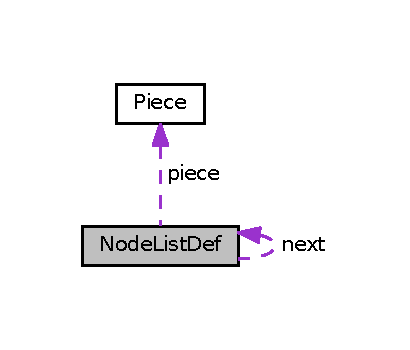
\includegraphics[width=197pt]{structNodeListDef__coll__graph}
\end{center}
\end{figure}
\subsection*{Pola danych}
\begin{DoxyCompactItemize}
\item 
\hypertarget{structNodeListDef_ab95b95938c8b32e30344bfb3bd943fa4}{\hyperlink{structPiece}{Piece} {\bfseries piece}}\label{structNodeListDef_ab95b95938c8b32e30344bfb3bd943fa4}

\item 
\hypertarget{structNodeListDef_a1344e8e757b2a2c029f7fb59fc34cd09}{\hyperlink{structNodeListDef}{Node\-List} $\ast$ {\bfseries next}}\label{structNodeListDef_a1344e8e757b2a2c029f7fb59fc34cd09}

\end{DoxyCompactItemize}


Dokumentacja dla tej struktury została wygenerowana z pliku\-:\begin{DoxyCompactItemize}
\item 
\hyperlink{ai_8c}{ai.\-c}\end{DoxyCompactItemize}

\hypertarget{structPiece}{\section{Dokumentacja struktury Piece}
\label{structPiece}\index{Piece@{Piece}}
}


Struct of \hyperlink{structPiece}{Piece}.  




{\ttfamily \#include $<$engine.\-h$>$}

\subsection*{Pola danych}
\begin{DoxyCompactItemize}
\item 
\hypertarget{structPiece_a895b6803ce74fe8574d6168d66ac6bb5}{int {\bfseries x}}\label{structPiece_a895b6803ce74fe8574d6168d66ac6bb5}

\item 
\hypertarget{structPiece_a97d61c9e42873e2274620c91178e879b}{int {\bfseries y}}\label{structPiece_a97d61c9e42873e2274620c91178e879b}

\item 
\hypertarget{structPiece_adbb6cdacb3b55e14dcf55152f1011fa4}{char {\bfseries ch}}\label{structPiece_adbb6cdacb3b55e14dcf55152f1011fa4}

\item 
\hypertarget{structPiece_a1ff878d1c3356c69814a5e18ef10aa18}{int {\bfseries turn\-Moved}}\label{structPiece_a1ff878d1c3356c69814a5e18ef10aa18}

\item 
\hypertarget{structPiece_ad1320904ecb8565e96d6020f857c990c}{bool {\bfseries moved}}\label{structPiece_ad1320904ecb8565e96d6020f857c990c}

\end{DoxyCompactItemize}


\subsection{Opis szczegółowy}
Struct of \hyperlink{structPiece}{Piece}. 


\begin{DoxyParams}{Parametry}
{\em x} & Number of column of a piece. \\
\hline
{\em y} & Number of row of a piece. \\
\hline
{\em ch} & Char representing a piece('K', 'C', 'R', 'k', 'c' or 'r') \\
\hline
{\em turn\-Moved} & Last turn this piece was moved. \\
\hline
{\em moved} & True if the piece was moved last turn. \\
\hline
\end{DoxyParams}


Dokumentacja dla tej struktury została wygenerowana z pliku\-:\begin{DoxyCompactItemize}
\item 
\hyperlink{engine_8h}{engine.\-h}\end{DoxyCompactItemize}

\hypertarget{structTreeNode}{\section{Dokumentacja struktury Tree\-Node}
\label{structTreeNode}\index{Tree\-Node@{Tree\-Node}}
}


Struct of a tree containing pieces.  




{\ttfamily \#include $<$engine.\-h$>$}



Diagram współpracy dla Tree\-Node\-:
\nopagebreak
\begin{figure}[H]
\begin{center}
\leavevmode
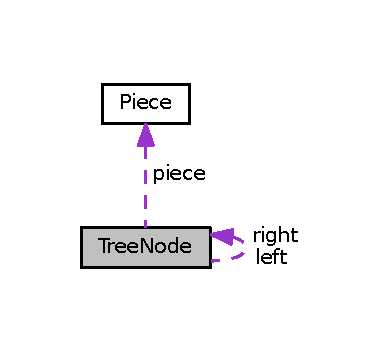
\includegraphics[width=184pt]{structTreeNode__coll__graph}
\end{center}
\end{figure}
\subsection*{Pola danych}
\begin{DoxyCompactItemize}
\item 
\hypertarget{structTreeNode_a3f2ec1b7aceb98384fe5a2096b63617f}{\hyperlink{structPiece}{Piece} {\bfseries piece}}\label{structTreeNode_a3f2ec1b7aceb98384fe5a2096b63617f}

\item 
\hypertarget{structTreeNode_af4ab5453a9305f5620c0eb9ac360fb90}{struct \hyperlink{structTreeNode}{Tree\-Node} $\ast$ {\bfseries left}}\label{structTreeNode_af4ab5453a9305f5620c0eb9ac360fb90}

\item 
\hypertarget{structTreeNode_ab36f951b4d3d53dfc2d345978900c6e2}{struct \hyperlink{structTreeNode}{Tree\-Node} $\ast$ {\bfseries right}}\label{structTreeNode_ab36f951b4d3d53dfc2d345978900c6e2}

\end{DoxyCompactItemize}


\subsection{Opis szczegółowy}
Struct of a tree containing pieces. 


\begin{DoxyParams}{Parametry}
{\em \hyperlink{structPiece}{Piece}} & Struct containing parameters of a \hyperlink{structPiece}{Piece} \\
\hline
\end{DoxyParams}
\begin{DoxySeeAlso}{Zobacz również}
\hyperlink{structPiece}{Piece} 
\end{DoxySeeAlso}

\begin{DoxyParams}{Parametry}
{\em left} & Pointer to left son of the node. \\
\hline
{\em right} & Pointer to right son of the node. \\
\hline
\end{DoxyParams}


Dokumentacja dla tej struktury została wygenerowana z pliku\-:\begin{DoxyCompactItemize}
\item 
\hyperlink{engine_8h}{engine.\-h}\end{DoxyCompactItemize}

\hypertarget{structVector}{\section{Dokumentacja struktury Vector}
\label{structVector}\index{Vector@{Vector}}
}
\subsection*{Pola danych}
\begin{DoxyCompactItemize}
\item 
\hypertarget{structVector_a14f004f4b3693f643b809d09249d09f4}{int {\bfseries X}}\label{structVector_a14f004f4b3693f643b809d09249d09f4}

\item 
\hypertarget{structVector_a159daaacad33412e58223190bead33e2}{int {\bfseries Y}}\label{structVector_a159daaacad33412e58223190bead33e2}

\end{DoxyCompactItemize}


Dokumentacja dla tej struktury została wygenerowana z pliku\-:\begin{DoxyCompactItemize}
\item 
\hyperlink{ai_8c}{ai.\-c}\end{DoxyCompactItemize}

\chapter{Dokumentacja plików}
\hypertarget{ai_8c}{\section{Dokumentacja pliku ai.\-c}
\label{ai_8c}\index{ai.\-c@{ai.\-c}}
}


Source file of A\-I.  


{\ttfamily \#include $<$stdio.\-h$>$}\\*
{\ttfamily \#include $<$assert.\-h$>$}\\*
{\ttfamily \#include $<$stdlib.\-h$>$}\\*
{\ttfamily \#include \char`\"{}ai.\-h\char`\"{}}\\*
Wykres zależności załączania dla ai.\-c\-:
\nopagebreak
\begin{figure}[H]
\begin{center}
\leavevmode
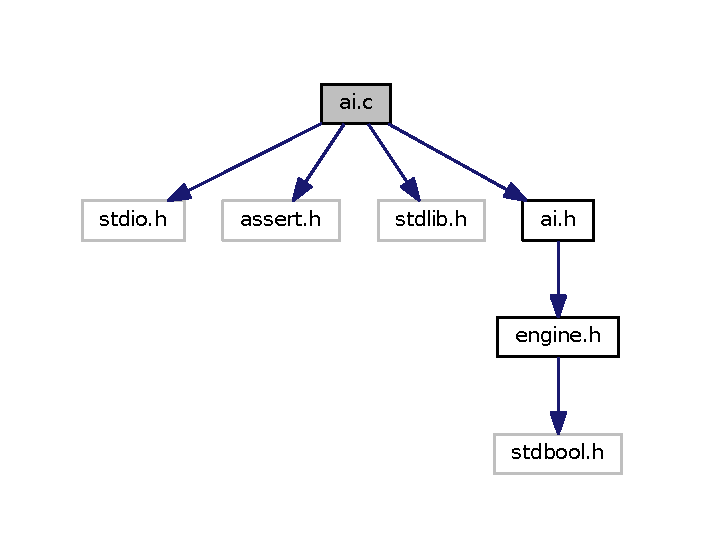
\includegraphics[width=338pt]{ai_8c__incl}
\end{center}
\end{figure}
\subsection*{Struktury danych}
\begin{DoxyCompactItemize}
\item 
struct \hyperlink{structVector}{Vector}
\item 
struct \hyperlink{structNodeListDef}{Node\-List\-Def}
\end{DoxyCompactItemize}
\subsection*{Definicje}
\begin{DoxyCompactItemize}
\item 
\hypertarget{ai_8c_a4fadfc1cc2d9a1723ae3ec08f3f0203d}{\#define {\bfseries N\-O\-R\-T\-H\-W\-E\-S\-T}~21}\label{ai_8c_a4fadfc1cc2d9a1723ae3ec08f3f0203d}

\item 
\hypertarget{ai_8c_a1711232abf72723b5216c206e6bbb175}{\#define {\bfseries N\-O\-R\-T\-H}~22}\label{ai_8c_a1711232abf72723b5216c206e6bbb175}

\item 
\hypertarget{ai_8c_a102c97a6b56626a25efbee52bc0ccff0}{\#define {\bfseries N\-O\-R\-T\-H\-E\-A\-S\-T}~23}\label{ai_8c_a102c97a6b56626a25efbee52bc0ccff0}

\item 
\hypertarget{ai_8c_a072a1ef1143314441742097b799be322}{\#define {\bfseries E\-A\-S\-T}~24}\label{ai_8c_a072a1ef1143314441742097b799be322}

\item 
\hypertarget{ai_8c_a0bdd815c79bee3fd7243675de570e3c4}{\#define {\bfseries S\-O\-U\-T\-H\-E\-A\-S\-T}~25}\label{ai_8c_a0bdd815c79bee3fd7243675de570e3c4}

\item 
\hypertarget{ai_8c_af3830320fe6287f717dca9669f417950}{\#define {\bfseries S\-O\-U\-T\-H}~26}\label{ai_8c_af3830320fe6287f717dca9669f417950}

\item 
\hypertarget{ai_8c_affb1a0defb8cb94cc31897c465e20a75}{\#define {\bfseries S\-O\-U\-T\-H\-W\-E\-S\-T}~27}\label{ai_8c_affb1a0defb8cb94cc31897c465e20a75}

\item 
\hypertarget{ai_8c_a755da365a2f771fdb9e15af22fee7d74}{\#define {\bfseries W\-E\-S\-T}~28}\label{ai_8c_a755da365a2f771fdb9e15af22fee7d74}

\end{DoxyCompactItemize}
\subsection*{Definicje typów}
\begin{DoxyCompactItemize}
\item 
\hypertarget{ai_8c_ab0412993a9e3f218f85f70474c80414c}{typedef struct \hyperlink{structNodeListDef}{Node\-List\-Def} {\bfseries Node\-List}}\label{ai_8c_ab0412993a9e3f218f85f70474c80414c}

\end{DoxyCompactItemize}
\subsection*{Funkcje}
\begin{DoxyCompactItemize}
\item 
\hypertarget{ai_8c_a7100b301f75832992efcb62fc2701091}{\hyperlink{structTreeNode}{Tree\-Node} $\ast$ {\bfseries find\-My\-Next\-Peasant} (\hyperlink{structTreeNode}{Tree\-Node} $\ast$$\ast$tree, int my\-Number, int turns)}\label{ai_8c_a7100b301f75832992efcb62fc2701091}

\item 
\hypertarget{ai_8c_a6caa90f21778b1facba361b2a25d9bcb}{\hyperlink{structTreeNode}{Tree\-Node} $\ast$ {\bfseries find\-My\-Next\-Not\-Moved\-Knight} (\hyperlink{structTreeNode}{Tree\-Node} $\ast$$\ast$tree, int my\-Number)}\label{ai_8c_a6caa90f21778b1facba361b2a25d9bcb}

\item 
\hypertarget{ai_8c_a5a037a4154eba49d8bae23ebe2f6042a}{\hyperlink{structTreeNode}{Tree\-Node} $\ast$ {\bfseries find\-King} (\hyperlink{structTreeNode}{Tree\-Node} $\ast$$\ast$tree, int my\-Number, bool my)}\label{ai_8c_a5a037a4154eba49d8bae23ebe2f6042a}

\item 
\hypertarget{ai_8c_a851a8857e834cfa1b29170300f440c5c}{void {\bfseries print\-All\-Pieces} (\hyperlink{structTreeNode}{Tree\-Node} $\ast$tree)}\label{ai_8c_a851a8857e834cfa1b29170300f440c5c}

\item 
\hypertarget{ai_8c_a5e0864d4fc7fa66f80a1f38a8b3d63ea}{bool {\bfseries this\-Piece\-Is\-Mine} (int my\-Number, char symbol)}\label{ai_8c_a5e0864d4fc7fa66f80a1f38a8b3d63ea}

\item 
\hypertarget{ai_8c_a3c7051b0b17c3545851226bc503d2fce}{bool {\bfseries its\-Closer\-Than\-Closest} (\hyperlink{structTreeNode}{Tree\-Node} $\ast$tree, \hyperlink{structTreeNode}{Tree\-Node} $\ast$closest, \hyperlink{structPiece}{Piece} my\-Piece, int my\-Number)}\label{ai_8c_a3c7051b0b17c3545851226bc503d2fce}

\item 
\hypertarget{ai_8c_a2140c1962bb7214d9b3629323377b893}{\hyperlink{structTreeNode}{Tree\-Node} $\ast$ {\bfseries closest\-Enemy} (\hyperlink{structTreeNode}{Tree\-Node} $\ast$tree, \hyperlink{structPiece}{Piece} my\-Piece, \hyperlink{structTreeNode}{Tree\-Node} $\ast$closest, int my\-Number)}\label{ai_8c_a2140c1962bb7214d9b3629323377b893}

\item 
\hypertarget{ai_8c_ab3cdee659431e48af1f96436ed1c17cf}{\hyperlink{structNodeListDef}{Node\-List} $\ast$ {\bfseries create\-My\-Units\-List} (\hyperlink{structTreeNode}{Tree\-Node} $\ast$$\ast$tree, char symbol, int my\-Number, int turns)}\label{ai_8c_ab3cdee659431e48af1f96436ed1c17cf}

\item 
\hypertarget{ai_8c_a6e3efb45a22a8fc130b186ce964f5421}{int {\bfseries list\-Size} (\hyperlink{structNodeListDef}{Node\-List} $\ast$list)}\label{ai_8c_a6e3efb45a22a8fc130b186ce964f5421}

\item 
\hypertarget{ai_8c_a12f4164db8c3b372c9dfa38ef5cd6eb8}{int {\bfseries define\-Direction} (\hyperlink{structPiece}{Piece} from, \hyperlink{structPiece}{Piece} to)}\label{ai_8c_a12f4164db8c3b372c9dfa38ef5cd6eb8}

\item 
\hypertarget{ai_8c_a65795ed21e57259c50fbc763f17e4417}{int {\bfseries find\-Best\-Direction} (int previous\-Direction, int $\ast$i)}\label{ai_8c_a65795ed21e57259c50fbc763f17e4417}

\item 
\hypertarget{ai_8c_a74e5e4f306a83f1b79bf6a4da428d413}{bool {\bfseries is\-On\-Pieces\-List} (int new\-X, int new\-Y, \hyperlink{structNodeListDef}{Node\-List} $\ast$my\-Pieces\-List)}\label{ai_8c_a74e5e4f306a83f1b79bf6a4da428d413}

\item 
\hypertarget{ai_8c_aac557f0cb03d289b4f1cadb3d77740c6}{void {\bfseries give\-New\-Coordinates} (int $\ast$new\-X, int $\ast$new\-Y, \hyperlink{structPiece}{Piece} piece, int direction, int n)}\label{ai_8c_aac557f0cb03d289b4f1cadb3d77740c6}

\item 
\hypertarget{ai_8c_a4f5900299ad4acc854780b066e5f8ada}{\hyperlink{structPiece}{Piece} {\bfseries try\-To\-Create\-New\-Piece} (\hyperlink{structTreeNode}{Tree\-Node} $\ast$$\ast$tree, \hyperlink{structNodeListDef}{Node\-List} $\ast$$\ast$my\-Peasants\-List, bool create\-Peasant, int direction, int n, int turns, int my\-Number)}\label{ai_8c_a4f5900299ad4acc854780b066e5f8ada}

\item 
\hypertarget{ai_8c_a9b83cf31cf9f44c124f5f6759deafb5d}{\hyperlink{structTreeNode}{Tree\-Node} $\ast$ {\bfseries produce\-Piece\-In\-Best\-Possible\-Square} (\hyperlink{structTreeNode}{Tree\-Node} $\ast$$\ast$tree, \hyperlink{structNodeListDef}{Node\-List} $\ast$$\ast$my\-Peasants\-List, bool \hyperlink{engine_8h_a610df406fe7f88d89ded2c1854c7d3aa}{produce\-Peasant}, int direction, int n, int turns, int my\-Number)}\label{ai_8c_a9b83cf31cf9f44c124f5f6759deafb5d}

\item 
\hypertarget{ai_8c_a72be22810c2f1e35df9934ea7bab1b08}{\hyperlink{structTreeNode}{Tree\-Node} $\ast$ {\bfseries produce\-New\-Pieces} (\hyperlink{structTreeNode}{Tree\-Node} $\ast$$\ast$tree, \hyperlink{structNodeListDef}{Node\-List} $\ast$$\ast$my\-Peasants\-List, bool \hyperlink{engine_8h_a610df406fe7f88d89ded2c1854c7d3aa}{produce\-Peasant}, int n, int turns, int my\-Num)}\label{ai_8c_a72be22810c2f1e35df9934ea7bab1b08}

\item 
\hypertarget{ai_8c_a552be12b88c3dca3cc46d2992e81ee28}{\hyperlink{structTreeNode}{Tree\-Node} $\ast$ {\bfseries try\-To\-Move\-Knight} (\hyperlink{structTreeNode}{Tree\-Node} $\ast$$\ast$tree, \hyperlink{structNodeListDef}{Node\-List} $\ast$$\ast$my\-Not\-Moved\-Knights\-List, int direction, int n, int my\-Number, bool $\ast$win)}\label{ai_8c_a552be12b88c3dca3cc46d2992e81ee28}

\item 
\hypertarget{ai_8c_ae8b974874f1ecf63fdd73691271ad9f5}{void {\bfseries delete\-List} (\hyperlink{structNodeListDef}{Node\-List} $\ast$$\ast$list)}\label{ai_8c_ae8b974874f1ecf63fdd73691271ad9f5}

\item 
\hypertarget{ai_8c_a2254d5c72fef018fbbbbfecc26e37c5c}{\hyperlink{structTreeNode}{Tree\-Node} $\ast$ {\bfseries move\-Knights} (\hyperlink{structTreeNode}{Tree\-Node} $\ast$$\ast$tree, \hyperlink{structNodeListDef}{Node\-List} $\ast$$\ast$knights\-List, int n, int my\-Number, bool $\ast$win)}\label{ai_8c_a2254d5c72fef018fbbbbfecc26e37c5c}

\item 
int \hyperlink{ai_8c_a14376896e70f2124b64debad28702f3b}{generate\-Action} (\hyperlink{structTreeNode}{Tree\-Node} $\ast$$\ast$tree, int $\ast$turns, bool $\ast$my\-Turn, int my\-Num, int n)
\begin{DoxyCompactList}\small\item\em A\-I generating all actions during current turn. \end{DoxyCompactList}\end{DoxyCompactItemize}


\subsection{Opis szczegółowy}
Source file of A\-I. Contains all necessary functions to genrate all actions during a turn. Some of these funtions can be exported and used in engine (both modules are independent). 

\subsection{Dokumentacja funkcji}
\hypertarget{ai_8c_a14376896e70f2124b64debad28702f3b}{\index{ai.\-c@{ai.\-c}!generate\-Action@{generate\-Action}}
\index{generate\-Action@{generate\-Action}!ai.c@{ai.\-c}}
\subsubsection[{generate\-Action}]{\setlength{\rightskip}{0pt plus 5cm}int generate\-Action (
\begin{DoxyParamCaption}
\item[{{\bf Tree\-Node} $\ast$$\ast$}]{tree, }
\item[{int $\ast$}]{turns, }
\item[{bool $\ast$}]{my\-Turn, }
\item[{int}]{my\-Num, }
\item[{int}]{n}
\end{DoxyParamCaption}
)}}\label{ai_8c_a14376896e70f2124b64debad28702f3b}


A\-I generating all actions during current turn. 

The function is an A\-I. It produces a peasant if player has only one unit of this type, otherwise produces a knight. It produces new units towards closest enemy piece. It also moves every knight towards closest enemy piece. If it cannot move or produce in this direction, tries to do it into neighbouring squares (until possible squares are further to closest enemy unit than peasant). Finally, it ends turn, decreasing parameter $\ast$turns (if player's number is 2), negates $\ast$my\-Turn and returns result.


\begin{DoxyParams}[1]{Parametry}
\mbox{\tt in,out}  & {\em $\ast$$\ast$tree} & Tree containing nodes with all pieces on board. \\
\hline
\mbox{\tt in,out}  & {\em $\ast$turns} & Number of remaining turns. \\
\hline
\mbox{\tt in,out}  & {\em $\ast$my\-Turn} & Parameter used in \hyperlink{middle__ages_8c}{middle\-\_\-ages.\-c} to define which turn it is\-: ai's (to generate action) or other player's (to parse his actions). Here only to be negated. \\
\hline
\mbox{\tt in}  & {\em my\-Num} & Player's number (1 or 2). \\
\hline
\mbox{\tt in}  & {\em n} & Size (of a side) of a board.\\
\hline
\end{DoxyParams}
\begin{DoxyReturn}{Zwraca}
Defined constant representing the result (W\-I\-N, D\-R\-A\-W, C\-O\-N\-T\-I\-N\-U\-E). 
\end{DoxyReturn}


Oto graf wywołań dla tej funkcji\-:
\nopagebreak
\begin{figure}[H]
\begin{center}
\leavevmode
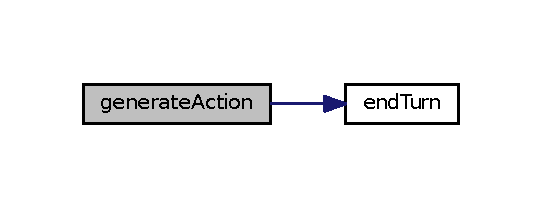
\includegraphics[width=260pt]{ai_8c_a14376896e70f2124b64debad28702f3b_cgraph}
\end{center}
\end{figure}



\hypertarget{ai_8h}{\section{Dokumentacja pliku ai.\-h}
\label{ai_8h}\index{ai.\-h@{ai.\-h}}
}


Interface of A\-I.  


{\ttfamily \#include \char`\"{}engine.\-h\char`\"{}}\\*
Wykres zależności załączania dla ai.\-h\-:
\nopagebreak
\begin{figure}[H]
\begin{center}
\leavevmode
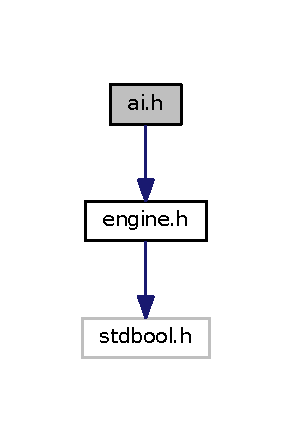
\includegraphics[width=140pt]{ai_8h__incl}
\end{center}
\end{figure}
Ten wykres pokazuje, które pliki bezpośrednio lub pośrednio załączają ten plik\-:
\nopagebreak
\begin{figure}[H]
\begin{center}
\leavevmode
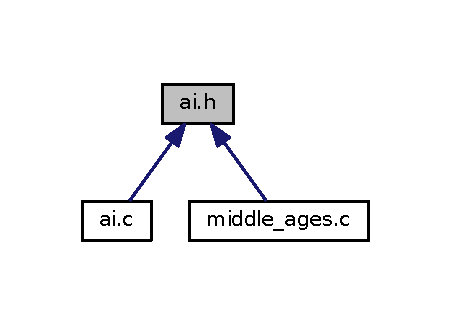
\includegraphics[width=217pt]{ai_8h__dep__incl}
\end{center}
\end{figure}
\subsection*{Funkcje}
\begin{DoxyCompactItemize}
\item 
int \hyperlink{ai_8h_a14376896e70f2124b64debad28702f3b}{generate\-Action} (\hyperlink{structTreeNode}{Tree\-Node} $\ast$$\ast$tree, int $\ast$turns, bool $\ast$my\-Turn, int my\-Num, int n)
\begin{DoxyCompactList}\small\item\em A\-I generating all actions during current turn. \end{DoxyCompactList}\end{DoxyCompactItemize}


\subsection{Opis szczegółowy}
Interface of A\-I. This A\-I is independent of \hyperlink{engine_8c}{engine.\-c}. Contains only one function, generate\-Action, which process all the turn (at a pinch modifies tree of pieces on board and other main variables) and returns proper result (represented by a constant). 

\subsection{Dokumentacja funkcji}
\hypertarget{ai_8h_a14376896e70f2124b64debad28702f3b}{\index{ai.\-h@{ai.\-h}!generate\-Action@{generate\-Action}}
\index{generate\-Action@{generate\-Action}!ai.h@{ai.\-h}}
\subsubsection[{generate\-Action}]{\setlength{\rightskip}{0pt plus 5cm}int generate\-Action (
\begin{DoxyParamCaption}
\item[{{\bf Tree\-Node} $\ast$$\ast$}]{tree, }
\item[{int $\ast$}]{turns, }
\item[{bool $\ast$}]{my\-Turn, }
\item[{int}]{my\-Num, }
\item[{int}]{n}
\end{DoxyParamCaption}
)}}\label{ai_8h_a14376896e70f2124b64debad28702f3b}


A\-I generating all actions during current turn. 

The function is an A\-I. It produces a peasant if player has only one unit of this type, otherwise produces a knight. It produces new units towards closest enemy piece. It also moves every knight towards closest enemy piece. If it cannot move or produce in this direction, tries to do it into neighbouring squares (until possible squares are further to closest enemy unit than peasant). Finally, it ends turn, decreasing parameter $\ast$turns (if player's number is 2), negates $\ast$my\-Turn and returns result.


\begin{DoxyParams}[1]{Parametry}
\mbox{\tt in,out}  & {\em $\ast$$\ast$tree} & Tree containing nodes with all pieces on board. \\
\hline
\mbox{\tt in,out}  & {\em $\ast$turns} & Number of remaining turns. \\
\hline
\mbox{\tt in,out}  & {\em $\ast$my\-Turn} & Parameter used in \hyperlink{middle__ages_8c}{middle\-\_\-ages.\-c} to define which turn it is\-: ai's (to generate action) or other player's (to parse his actions). Here only to be negated. \\
\hline
\mbox{\tt in}  & {\em my\-Num} & Player's number (1 or 2). \\
\hline
\mbox{\tt in}  & {\em n} & Size (of a side) of a board.\\
\hline
\end{DoxyParams}
\begin{DoxyReturn}{Zwraca}
Defined constant representing the result (W\-I\-N, D\-R\-A\-W, C\-O\-N\-T\-I\-N\-U\-E). 
\end{DoxyReturn}


Oto graf wywołań dla tej funkcji\-:
\nopagebreak
\begin{figure}[H]
\begin{center}
\leavevmode
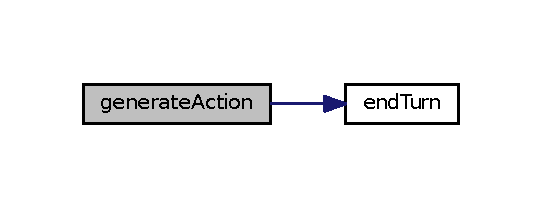
\includegraphics[width=260pt]{ai_8h_a14376896e70f2124b64debad28702f3b_cgraph}
\end{center}
\end{figure}



\hypertarget{engine_8c}{\section{Dokumentacja pliku engine.\-c}
\label{engine_8c}\index{engine.\-c@{engine.\-c}}
}


Source code of engine of a game.  


{\ttfamily \#include $<$stdio.\-h$>$}\\*
{\ttfamily \#include $<$stdlib.\-h$>$}\\*
{\ttfamily \#include $<$stdbool.\-h$>$}\\*
{\ttfamily \#include $<$assert.\-h$>$}\\*
{\ttfamily \#include \char`\"{}engine.\-h\char`\"{}}\\*
Wykres zależności załączania dla engine.\-c\-:
\nopagebreak
\begin{figure}[H]
\begin{center}
\leavevmode
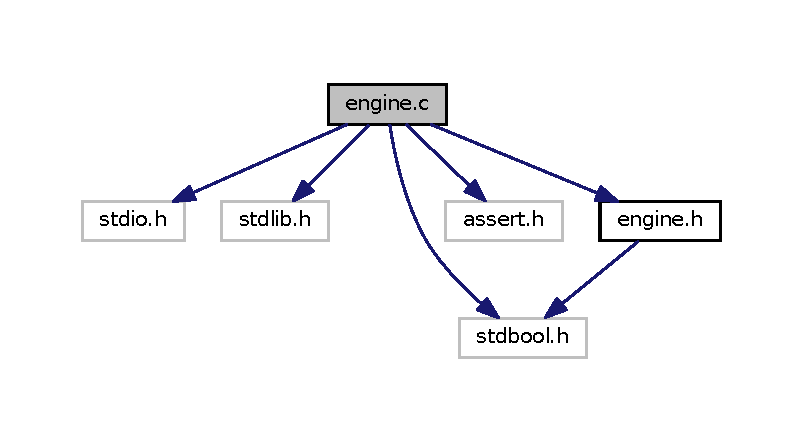
\includegraphics[width=350pt]{engine_8c__incl}
\end{center}
\end{figure}
\subsection*{Definicje}
\begin{DoxyCompactItemize}
\item 
\hypertarget{engine_8c_a2a37b4217917105aac7557862ccc19c3}{\#define {\bfseries M\-A\-X\-S\-I\-Z\-E}~2147483647}\label{engine_8c_a2a37b4217917105aac7557862ccc19c3}

\item 
\hypertarget{engine_8c_ab711666ad09d7f6c0b91576525ea158e}{\#define {\bfseries C\-O\-N\-T\-I\-N\-U\-E}~3}\label{engine_8c_ab711666ad09d7f6c0b91576525ea158e}

\item 
\hypertarget{engine_8c_a288116f92845fddefeb044f5b84bc889}{\#define {\bfseries I\-N\-P\-U\-T\-\_\-\-E\-R\-R\-O\-R}~42}\label{engine_8c_a288116f92845fddefeb044f5b84bc889}

\item 
\hypertarget{engine_8c_a7a7cd353a6274e8c0dbb698113e7e194}{\#define {\bfseries D\-R\-A\-W}~1}\label{engine_8c_a7a7cd353a6274e8c0dbb698113e7e194}

\item 
\hypertarget{engine_8c_a2199bc4c776dbd7a4248aeef9e5dd8a1}{\#define {\bfseries D\-R\-A\-W\-\_\-\-A\-F\-T\-E\-R\-\_\-\-E\-N\-D\-\_\-\-T\-U\-R\-N}~5}\label{engine_8c_a2199bc4c776dbd7a4248aeef9e5dd8a1}

\item 
\hypertarget{engine_8c_a6ee3d6fa4e432d9456967fd82533de48}{\#define {\bfseries E\-N\-D\-\_\-\-T\-U\-R\-N}~6}\label{engine_8c_a6ee3d6fa4e432d9456967fd82533de48}

\item 
\hypertarget{engine_8c_a4db4e218f5d127d392593464377e7dbe}{\#define {\bfseries P1\-\_\-\-W\-I\-N}~7}\label{engine_8c_a4db4e218f5d127d392593464377e7dbe}

\item 
\hypertarget{engine_8c_a4081f92247bfc37403cab4610a4681a0}{\#define {\bfseries P2\-\_\-\-W\-I\-N}~8}\label{engine_8c_a4081f92247bfc37403cab4610a4681a0}

\item 
\hypertarget{engine_8c_a43105771f16e2da3078149f0de528e9b}{\#define {\bfseries W\-I\-N}~0}\label{engine_8c_a43105771f16e2da3078149f0de528e9b}

\item 
\hypertarget{engine_8c_a0d781d111f2907153eb8fd334b4495eb}{\#define {\bfseries L\-O\-S\-T}~2}\label{engine_8c_a0d781d111f2907153eb8fd334b4495eb}

\item 
\hypertarget{engine_8c_a5d2cfa5bf999d10fd3cb4490e96b6c2e}{\#define {\bfseries D\-R\-A\-W\-\_\-\-B\-U\-T\-\_\-\-F\-I\-R\-S\-T\-\_\-\-P\-L\-A\-Y\-E\-R\-\_\-\-R\-E\-A\-D\-S\-\_\-\-L\-A\-S\-T\-\_\-\-I\-N\-P\-U\-T}~9}\label{engine_8c_a5d2cfa5bf999d10fd3cb4490e96b6c2e}

\end{DoxyCompactItemize}
\subsection*{Funkcje}
\begin{DoxyCompactItemize}
\item 
\hypertarget{engine_8c_a49fb4e958411b1184e861188373973a2}{void {\bfseries deallocate\-Tree} (\hyperlink{structTreeNode}{Tree\-Node} $\ast$node)}\label{engine_8c_a49fb4e958411b1184e861188373973a2}

\item 
\hyperlink{structPiece}{Piece} \hyperlink{engine_8c_a569bd36a50e0153fc11b045c0403ea13}{create\-Piece} (int x, int y, char ch, int turns, bool my\-Turn, int my\-Number)
\begin{DoxyCompactList}\small\item\em Creates piece of given parameters. \end{DoxyCompactList}\item 
\hypertarget{engine_8c_a7a5d69dbc08b9c58392c4ef15ed1a648}{\hyperlink{structTreeNode}{Tree\-Node} $\ast$ {\bfseries create\-Node} (\hyperlink{structPiece}{Piece} piece)}\label{engine_8c_a7a5d69dbc08b9c58392c4ef15ed1a648}

\item 
\hypertarget{engine_8c_aab281c58fb42fa5d2b8008ef0894a012}{int {\bfseries compare\-Num} (int x1, int y1, int x2, int y2)}\label{engine_8c_aab281c58fb42fa5d2b8008ef0894a012}

\item 
\hyperlink{structTreeNode}{Tree\-Node} $\ast$ \hyperlink{engine_8c_af2a455cb77697f2c6c4ad4fa0479d8ee}{insert\-Element} (\hyperlink{structTreeNode}{Tree\-Node} $\ast$root, char $\ast$$\ast$board, int m, \hyperlink{structPiece}{Piece} piece)
\begin{DoxyCompactList}\small\item\em Iterative insertion of a new node cointaining given piece into tree. \end{DoxyCompactList}\item 
\hypertarget{engine_8c_ac7c6e612a87e3989e4c8c93f54365c14}{\hyperlink{structPiece}{Piece} {\bfseries find\-Min} (\hyperlink{structTreeNode}{Tree\-Node} $\ast$node)}\label{engine_8c_ac7c6e612a87e3989e4c8c93f54365c14}

\item 
\hyperlink{structTreeNode}{Tree\-Node} $\ast$ \hyperlink{engine_8c_a407d2933a52398d81878fab4e6ca44a6}{delete\-Node} (\hyperlink{structPiece}{Piece} piece, \hyperlink{structTreeNode}{Tree\-Node} $\ast$$\ast$node)
\begin{DoxyCompactList}\small\item\em Recursive removal of node containing given piece from tree. \end{DoxyCompactList}\item 
\hypertarget{engine_8c_ad7fae91a72df85088458207f52c72cf3}{void {\bfseries reset\-Pieces} (\hyperlink{structTreeNode}{Tree\-Node} $\ast$node, int turns)}\label{engine_8c_ad7fae91a72df85088458207f52c72cf3}

\item 
void \hyperlink{engine_8c_a0776cd662f5c945bb00f5950ab384fcf}{start\-Game} (\hyperlink{structTreeNode}{Tree\-Node} $\ast$$\ast$tree)
\begin{DoxyCompactList}\small\item\em Initializes a game. \end{DoxyCompactList}\item 
\hypertarget{engine_8c_a2a1992511421b3e7a9b132416073ed92}{void {\bfseries print\-Result} (int $\ast$result, int my\-Number)}\label{engine_8c_a2a1992511421b3e7a9b132416073ed92}

\item 
\hypertarget{engine_8c_af48aaea8890f91928dc4fb6c14f6f5c6}{void {\bfseries deallocate\-Memory} (char $\ast$$\ast$$\ast$board, int m)}\label{engine_8c_af48aaea8890f91928dc4fb6c14f6f5c6}

\item 
void \hyperlink{engine_8c_a9d28173fc9942b170570a3be404f5d82}{end\-Game} (\hyperlink{structTreeNode}{Tree\-Node} $\ast$$\ast$node, int $\ast$result, char $\ast$$\ast$$\ast$board, int m, int my\-Number)
\begin{DoxyCompactList}\small\item\em Frees memory. \end{DoxyCompactList}\item 
int \hyperlink{engine_8c_abd8bbcfabb3ddef2ccaafb9928a37b95}{min} (int a, int b)
\begin{DoxyCompactList}\small\item\em Returns lesser value of two ints. \end{DoxyCompactList}\item 
\hypertarget{engine_8c_af082905f7eac6d03e92015146bbc1925}{int {\bfseries max} (int a, int b)}\label{engine_8c_af082905f7eac6d03e92015146bbc1925}

\item 
\hypertarget{engine_8c_a6e6eb7483b9489c5387b8e941b1c0a25}{int {\bfseries metric} (int x1, int y1, int x2, int y2)}\label{engine_8c_a6e6eb7483b9489c5387b8e941b1c0a25}

\item 
int \hyperlink{engine_8c_aaa9b56690bf5f53d7d72d2e76d7ff74d}{metric\-Min} (int x1, int y1, int x2, int y2)
\begin{DoxyCompactList}\small\item\em Finds lesser of two distances\-: between x or y coordinates. \end{DoxyCompactList}\item 
char $\ast$$\ast$ \hyperlink{engine_8c_a6e2f079a3de8efe3d5d507181cee3153}{allocate\-Memory} (int m)
\begin{DoxyCompactList}\small\item\em Allocates space for m by m array and fills it with dot. \end{DoxyCompactList}\item 
int \hyperlink{engine_8c_ad928eca8b7bb809339cc97d651092d47}{assign\-Symbol} (int my\-Number, bool my, char symbol)
\begin{DoxyCompactList}\small\item\em Function used to return symbol of particular unit type of given player. \end{DoxyCompactList}\item 
\hypertarget{engine_8c_af831765909b7fd39a171d81035bc135b}{void {\bfseries put\-Tree\-On\-Board} (\hyperlink{structTreeNode}{Tree\-Node} $\ast$node, char $\ast$$\ast$board, int m)}\label{engine_8c_af831765909b7fd39a171d81035bc135b}

\item 
void \hyperlink{engine_8c_ab1554076e8bcda9021d6a6273c21af4c}{print\-Topleft} (char $\ast$$\ast$board, int m)
\begin{DoxyCompactList}\small\item\em Prints (into stdout) top-\/left corner of the board of size m x m. \end{DoxyCompactList}\item 
\hyperlink{structTreeNode}{Tree\-Node} $\ast$ \hyperlink{engine_8c_a5b4106f2297731d094d9ef72d2a7e652}{find\-Node} (int x, int y, \hyperlink{structTreeNode}{Tree\-Node} $\ast$node)
\begin{DoxyCompactList}\small\item\em Searches tree for node containing a piece of given x and y. \end{DoxyCompactList}\item 
int \hyperlink{engine_8c_af5b804d6459b20c0bb9c976e720d8a25}{init} (int n, int k, int p, int x1, int y1, int x2, int y2, \hyperlink{structTreeNode}{Tree\-Node} $\ast$$\ast$tree, int $\ast$n\-My, int $\ast$k\-My, int $\ast$player\-Number, char $\ast$$\ast$board, int $\ast$m)
\begin{DoxyCompactList}\small\item\em Initializes a game with size of a board, number of rounds and positions of kings. \end{DoxyCompactList}\item 
\hypertarget{engine_8c_a3035ab21dcb74c46517b1f5af4c62565}{int {\bfseries move\-On\-Unoccupied\-Square} (\hyperlink{structTreeNode}{Tree\-Node} $\ast$moved, \hyperlink{structTreeNode}{Tree\-Node} $\ast$$\ast$tree, int x, int y, char $\ast$$\ast$board, int m, int turns)}\label{engine_8c_a3035ab21dcb74c46517b1f5af4c62565}

\item 
\hypertarget{engine_8c_a9c4f32052aeffa080f10e7385d0ef3e6}{bool {\bfseries check\-Owner} (\hyperlink{structPiece}{Piece} piece, bool my\-Turn, int my\-Number, bool moved)}\label{engine_8c_a9c4f32052aeffa080f10e7385d0ef3e6}

\item 
\hypertarget{engine_8c_a6420681a4fcf7c5e603642ecf108a5b6}{int {\bfseries move\-On\-Occupied\-Square} (\hyperlink{structTreeNode}{Tree\-Node} $\ast$moved\-\_\-node, \hyperlink{structTreeNode}{Tree\-Node} $\ast$beaten\-\_\-node, \hyperlink{structTreeNode}{Tree\-Node} $\ast$$\ast$tree, bool my\-Turn, int my\-Number, char $\ast$$\ast$board, int m, int turns)}\label{engine_8c_a6420681a4fcf7c5e603642ecf108a5b6}

\item 
\hypertarget{engine_8c_a6401bb44e7575a16f5afc9f0915d9131}{bool {\bfseries check\-Params} (int x1, int y1, int x2, int y2, int n)}\label{engine_8c_a6401bb44e7575a16f5afc9f0915d9131}

\item 
int \hyperlink{engine_8c_a17be2b87232c11cc093398d574452aa5}{move} (int x1, int y1, int x2, int y2, int n, bool my\-Turn, \hyperlink{structTreeNode}{Tree\-Node} $\ast$$\ast$tree, char $\ast$$\ast$board, int m, int turns, int my\-Number)
\begin{DoxyCompactList}\small\item\em Makes a move. \end{DoxyCompactList}\item 
\hypertarget{engine_8c_a22d64b3ee551798dfe3225afd4892f5f}{int {\bfseries produce\-Piece} (char piece, int x1, int y1, int x2, int y2, int n, bool my\-Turn, int my\-Number, \hyperlink{structTreeNode}{Tree\-Node} $\ast$$\ast$tree, char $\ast$$\ast$board, int m, int turns)}\label{engine_8c_a22d64b3ee551798dfe3225afd4892f5f}

\item 
int \hyperlink{engine_8c_ac274a9b90ffa3c10e8c9ef7ae2ca98c6}{produce\-Knight} (int x1, int y1, int x2, int y2, int n, bool my\-Turn, int my\-Number, \hyperlink{structTreeNode}{Tree\-Node} $\ast$$\ast$tree, char $\ast$$\ast$board, int m, int turns)
\begin{DoxyCompactList}\small\item\em Produces a knight. \end{DoxyCompactList}\item 
int \hyperlink{engine_8c_a610df406fe7f88d89ded2c1854c7d3aa}{produce\-Peasant} (int x1, int y1, int x2, int y2, int n, bool my\-Turn, int my\-Number, \hyperlink{structTreeNode}{Tree\-Node} $\ast$$\ast$tree, char $\ast$$\ast$board, int m, int turns)
\begin{DoxyCompactList}\small\item\em Produces a peasant. \end{DoxyCompactList}\item 
int \hyperlink{engine_8c_ad4a9988f23de955ff7858d69f6738f38}{end\-Turn} (int $\ast$turns, bool $\ast$my\-Turn, int my\-Number, \hyperlink{structTreeNode}{Tree\-Node} $\ast$tree, bool win)
\begin{DoxyCompactList}\small\item\em Ends a turn. \end{DoxyCompactList}\end{DoxyCompactItemize}


\subsection{Opis szczegółowy}
Source code of engine of a game. Contains all necessary functions to start, play, check arguments from input, and end a game. 

\subsection{Dokumentacja funkcji}
\hypertarget{engine_8c_a6e2f079a3de8efe3d5d507181cee3153}{\index{engine.\-c@{engine.\-c}!allocate\-Memory@{allocate\-Memory}}
\index{allocate\-Memory@{allocate\-Memory}!engine.c@{engine.\-c}}
\subsubsection[{allocate\-Memory}]{\setlength{\rightskip}{0pt plus 5cm}char$\ast$$\ast$ allocate\-Memory (
\begin{DoxyParamCaption}
\item[{int}]{m}
\end{DoxyParamCaption}
)}}\label{engine_8c_a6e2f079a3de8efe3d5d507181cee3153}


Allocates space for m by m array and fills it with dot. 


\begin{DoxyParams}[1]{Parametry}
\mbox{\tt in}  & {\em m} & Size of the array. \\
\hline
\end{DoxyParams}
\begin{DoxyReturn}{Zwraca}
allocated array 
\end{DoxyReturn}
\hypertarget{engine_8c_ad928eca8b7bb809339cc97d651092d47}{\index{engine.\-c@{engine.\-c}!assign\-Symbol@{assign\-Symbol}}
\index{assign\-Symbol@{assign\-Symbol}!engine.c@{engine.\-c}}
\subsubsection[{assign\-Symbol}]{\setlength{\rightskip}{0pt plus 5cm}int assign\-Symbol (
\begin{DoxyParamCaption}
\item[{int}]{my\-Number, }
\item[{bool}]{my, }
\item[{char}]{symbol}
\end{DoxyParamCaption}
)}}\label{engine_8c_ad928eca8b7bb809339cc97d651092d47}


Function used to return symbol of particular unit type of given player. 


\begin{DoxyParams}[1]{Parametry}
\mbox{\tt in}  & {\em my\-Number} & Number of player calling this function. \\
\hline
\mbox{\tt in}  & {\em my} & Logical value describing if caller wants to know his or opponent's unit's symbol. (used to avoid long ugly my\-Number == 1 ? 1 \-: 2 in first parameter) \\
\hline
\mbox{\tt in}  & {\em symbol} & Character describing symbol of which unit we want to be returned ('K', 'C' or 'R').\\
\hline
\end{DoxyParams}
\begin{DoxyReturn}{Zwraca}
Symbol (int value of character) of given player's unit. 
\end{DoxyReturn}
\hypertarget{engine_8c_a569bd36a50e0153fc11b045c0403ea13}{\index{engine.\-c@{engine.\-c}!create\-Piece@{create\-Piece}}
\index{create\-Piece@{create\-Piece}!engine.c@{engine.\-c}}
\subsubsection[{create\-Piece}]{\setlength{\rightskip}{0pt plus 5cm}{\bf Piece} create\-Piece (
\begin{DoxyParamCaption}
\item[{int}]{x, }
\item[{int}]{y, }
\item[{char}]{ch, }
\item[{int}]{turns, }
\item[{bool}]{my\-Turn, }
\item[{int}]{my\-Number}
\end{DoxyParamCaption}
)}}\label{engine_8c_a569bd36a50e0153fc11b045c0403ea13}


Creates piece of given parameters. 


\begin{DoxyParams}[1]{Parametry}
\mbox{\tt in}  & {\em x} & First coordinate of a new piece. \\
\hline
\mbox{\tt in}  & {\em y} & Second coordinate of a new piece \\
\hline
\mbox{\tt in}  & {\em ch} & Symbol (K, C or R) of a new piece. \\
\hline
\mbox{\tt in}  & {\em turns} & Remaining number of turns to describe when piece was moved. \\
\hline
\mbox{\tt in}  & {\em my\-Turn} & True if current turn is player's calling this function. \\
\hline
\mbox{\tt in}  & {\em my\-Number} & Number (1 or 2) of player calling this function (to define symbol of new piece, ex. 'K' or 'k'.\\
\hline
\end{DoxyParams}
\begin{DoxyReturn}{Zwraca}
Created piece. 
\end{DoxyReturn}


Oto graf wywoływań tej funkcji\-:
\nopagebreak
\begin{figure}[H]
\begin{center}
\leavevmode
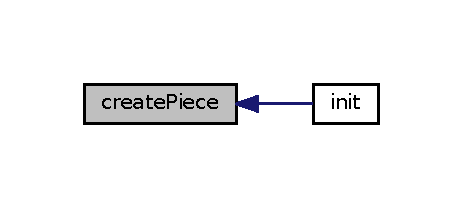
\includegraphics[width=222pt]{engine_8c_a569bd36a50e0153fc11b045c0403ea13_icgraph}
\end{center}
\end{figure}


\hypertarget{engine_8c_a407d2933a52398d81878fab4e6ca44a6}{\index{engine.\-c@{engine.\-c}!delete\-Node@{delete\-Node}}
\index{delete\-Node@{delete\-Node}!engine.c@{engine.\-c}}
\subsubsection[{delete\-Node}]{\setlength{\rightskip}{0pt plus 5cm}{\bf Tree\-Node}$\ast$ delete\-Node (
\begin{DoxyParamCaption}
\item[{{\bf Piece}}]{piece, }
\item[{{\bf Tree\-Node} $\ast$$\ast$}]{node}
\end{DoxyParamCaption}
)}}\label{engine_8c_a407d2933a52398d81878fab4e6ca44a6}


Recursive removal of node containing given piece from tree. 


\begin{DoxyParams}[1]{Parametry}
\mbox{\tt in}  & {\em piece} & A piece that is to be removed. \\
\hline
\mbox{\tt in,out}  & {\em node} & Root of tree containing piece to remove.\\
\hline
\end{DoxyParams}
\begin{DoxyReturn}{Zwraca}
Modified tree (passed with $\ast$$\ast$node) without removed node. 
\end{DoxyReturn}


Oto graf wywołań dla tej funkcji\-:
\nopagebreak
\begin{figure}[H]
\begin{center}
\leavevmode
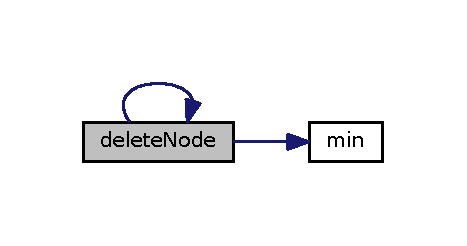
\includegraphics[width=224pt]{engine_8c_a407d2933a52398d81878fab4e6ca44a6_cgraph}
\end{center}
\end{figure}




Oto graf wywoływań tej funkcji\-:
\nopagebreak
\begin{figure}[H]
\begin{center}
\leavevmode
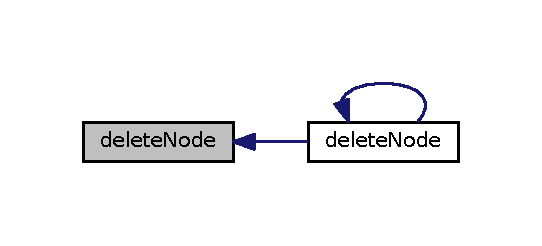
\includegraphics[width=260pt]{engine_8c_a407d2933a52398d81878fab4e6ca44a6_icgraph}
\end{center}
\end{figure}


\hypertarget{engine_8c_a9d28173fc9942b170570a3be404f5d82}{\index{engine.\-c@{engine.\-c}!end\-Game@{end\-Game}}
\index{end\-Game@{end\-Game}!engine.c@{engine.\-c}}
\subsubsection[{end\-Game}]{\setlength{\rightskip}{0pt plus 5cm}void end\-Game (
\begin{DoxyParamCaption}
\item[{{\bf Tree\-Node} $\ast$$\ast$}]{tree, }
\item[{int $\ast$}]{result, }
\item[{char $\ast$$\ast$$\ast$}]{board, }
\item[{int}]{m, }
\item[{int}]{my\-Number}
\end{DoxyParamCaption}
)}}\label{engine_8c_a9d28173fc9942b170570a3be404f5d82}


Frees memory. 

Needed after finishing game.


\begin{DoxyParams}[1]{Parametry}
\mbox{\tt in,out}  & {\em tree} & Tree containing nodes with all existing pieces. \\
\hline
\mbox{\tt out}  & {\em result} & Variable keeping result of the game so that proper output can be printed. Also changed to 0 or 42 and returned in main function. \\
\hline
\mbox{\tt in,out}  & {\em board} & Array representing top left part of a board. \\
\hline
\mbox{\tt in}  & {\em m} & Size of board. \\
\hline
\mbox{\tt in}  & {\em my\-Number} & Caller player number (1 or 2). \\
\hline
\end{DoxyParams}
\hypertarget{engine_8c_ad4a9988f23de955ff7858d69f6738f38}{\index{engine.\-c@{engine.\-c}!end\-Turn@{end\-Turn}}
\index{end\-Turn@{end\-Turn}!engine.c@{engine.\-c}}
\subsubsection[{end\-Turn}]{\setlength{\rightskip}{0pt plus 5cm}int end\-Turn (
\begin{DoxyParamCaption}
\item[{int $\ast$}]{turns, }
\item[{bool $\ast$}]{my\-Turn, }
\item[{int}]{my\-Number, }
\item[{{\bf Tree\-Node} $\ast$}]{tree, }
\item[{bool}]{win}
\end{DoxyParamCaption}
)}}\label{engine_8c_ad4a9988f23de955ff7858d69f6738f38}


Ends a turn. 

Changes current player. Checks if both players ended their turns, then \char`\"{}refreshes\char`\"{} all pieces before next turn and changes and decreases remaining number of turns.


\begin{DoxyParams}[1]{Parametry}
\mbox{\tt in,out}  & {\em turns} & Number of remaining turns. \\
\hline
\mbox{\tt in,out}  & {\em players1\-Turn} & Informs if turn being ended was player 1's. \\
\hline
\mbox{\tt in,out}  & {\em tree} & Tree containing nodes with all existing pieces. \\
\hline
\mbox{\tt in}  & {\em p1\-Initialized} & Information if I\-N\-I\-T of the first player has already been called. \\
\hline
\mbox{\tt in}  & {\em p2\-Initialized} & Information if I\-N\-I\-T of the second player has already been called. \\
\hline
\mbox{\tt in}  & {\em win} & Logical value used by A\-I if it beat opponent's king.\\
\hline
\end{DoxyParams}
\begin{DoxyReturn}{Zwraca}
Result depending on process of last turn (ex. P1\-\_\-\-W\-I\-N, D\-R\-A\-W etc.) 
\end{DoxyReturn}


Oto graf wywoływań tej funkcji\-:
\nopagebreak
\begin{figure}[H]
\begin{center}
\leavevmode
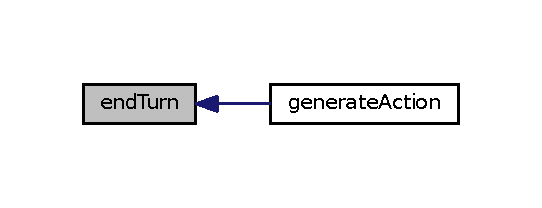
\includegraphics[width=260pt]{engine_8c_ad4a9988f23de955ff7858d69f6738f38_icgraph}
\end{center}
\end{figure}


\hypertarget{engine_8c_a5b4106f2297731d094d9ef72d2a7e652}{\index{engine.\-c@{engine.\-c}!find\-Node@{find\-Node}}
\index{find\-Node@{find\-Node}!engine.c@{engine.\-c}}
\subsubsection[{find\-Node}]{\setlength{\rightskip}{0pt plus 5cm}{\bf Tree\-Node}$\ast$ find\-Node (
\begin{DoxyParamCaption}
\item[{int}]{x, }
\item[{int}]{y, }
\item[{{\bf Tree\-Node} $\ast$}]{node}
\end{DoxyParamCaption}
)}}\label{engine_8c_a5b4106f2297731d094d9ef72d2a7e652}


Searches tree for node containing a piece of given x and y. 


\begin{DoxyParams}[1]{Parametry}
\mbox{\tt in}  & {\em x} & First coordinate of piece that is looked for. \\
\hline
\mbox{\tt in}  & {\em y} & Second coordinate of piece that is looked for. \\
\hline
\mbox{\tt in}  & {\em node} & Tree containing nodes with all pieces.\\
\hline
\end{DoxyParams}
\begin{DoxyReturn}{Zwraca}
found node or N\-U\-L\-L. 
\end{DoxyReturn}


Oto graf wywoływań tej funkcji\-:
\nopagebreak
\begin{figure}[H]
\begin{center}
\leavevmode
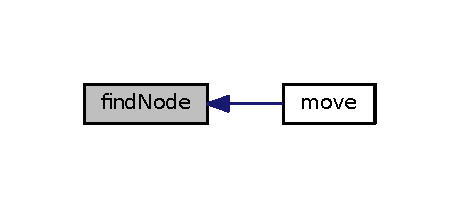
\includegraphics[width=220pt]{engine_8c_a5b4106f2297731d094d9ef72d2a7e652_icgraph}
\end{center}
\end{figure}


\hypertarget{engine_8c_af5b804d6459b20c0bb9c976e720d8a25}{\index{engine.\-c@{engine.\-c}!init@{init}}
\index{init@{init}!engine.c@{engine.\-c}}
\subsubsection[{init}]{\setlength{\rightskip}{0pt plus 5cm}int init (
\begin{DoxyParamCaption}
\item[{int}]{n, }
\item[{int}]{k, }
\item[{int}]{p, }
\item[{int}]{x1, }
\item[{int}]{y1, }
\item[{int}]{x2, }
\item[{int}]{y2, }
\item[{{\bf Tree\-Node} $\ast$$\ast$}]{tree, }
\item[{int $\ast$}]{n\-My, }
\item[{int $\ast$}]{k\-My, }
\item[{int $\ast$}]{player\-Number, }
\item[{char $\ast$$\ast$}]{board, }
\item[{int $\ast$}]{m}
\end{DoxyParamCaption}
)}}\label{engine_8c_af5b804d6459b20c0bb9c976e720d8a25}


Initializes a game with size of a board, number of rounds and positions of kings. 

One I\-N\-I\-T for each player is needed before any other command.


\begin{DoxyParams}[1]{Parametry}
\mbox{\tt in}  & {\em n} & Size of a board. \\
\hline
\mbox{\tt in}  & {\em k} & Number of turns of each player. \\
\hline
\mbox{\tt in}  & {\em p} & Number of player for whom initialization is called. \\
\hline
\mbox{\tt in}  & {\em x1} & Column number of first player's king. \\
\hline
\mbox{\tt in}  & {\em y1} & Row number of first player's king. \\
\hline
\mbox{\tt in}  & {\em x2} & Column number of second player's king. \\
\hline
\mbox{\tt in}  & {\em y2} & Row number of second player's king. \\
\hline
\mbox{\tt in,out}  & {\em tree} & Tree containing nodes with all existing pieces. \\
\hline
\mbox{\tt out}  & {\em n\-My} & Variable keeping the size of board. \\
\hline
\mbox{\tt out}  & {\em k\-My} & Variable keeping number of turns. \\
\hline
\mbox{\tt in}  & {\em p1\-Initialized} & Information if I\-N\-I\-T of the first player has already been called. \\
\hline
\mbox{\tt in}  & {\em p2\-Initialized} & Information if I\-N\-I\-T of the second player has already been called. \\
\hline
\mbox{\tt in,out}  & {\em board} & Array representing top left part of a board. \\
\hline
\mbox{\tt in}  & {\em m} & Size of board.\\
\hline
\end{DoxyParams}
\begin{DoxyReturn}{Zwraca}
C\-O\-N\-T\-I\-N\-U\-E if all arguments were correct. 

I\-N\-P\-U\-T\-\_\-\-E\-R\-R\-O\-R if there was an input error. 
\end{DoxyReturn}


Oto graf wywołań dla tej funkcji\-:
\nopagebreak
\begin{figure}[H]
\begin{center}
\leavevmode
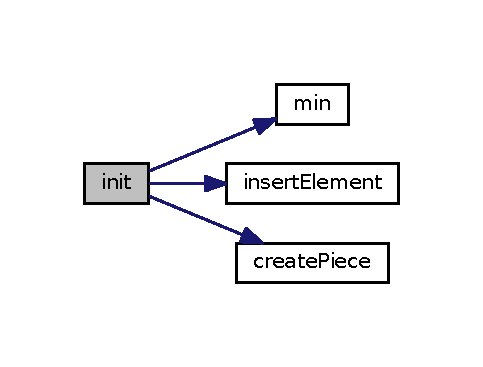
\includegraphics[width=232pt]{engine_8c_af5b804d6459b20c0bb9c976e720d8a25_cgraph}
\end{center}
\end{figure}


\hypertarget{engine_8c_af2a455cb77697f2c6c4ad4fa0479d8ee}{\index{engine.\-c@{engine.\-c}!insert\-Element@{insert\-Element}}
\index{insert\-Element@{insert\-Element}!engine.c@{engine.\-c}}
\subsubsection[{insert\-Element}]{\setlength{\rightskip}{0pt plus 5cm}{\bf Tree\-Node}$\ast$ insert\-Element (
\begin{DoxyParamCaption}
\item[{{\bf Tree\-Node} $\ast$}]{root, }
\item[{char $\ast$$\ast$}]{board, }
\item[{int}]{m, }
\item[{{\bf Piece}}]{piece}
\end{DoxyParamCaption}
)}}\label{engine_8c_af2a455cb77697f2c6c4ad4fa0479d8ee}


Iterative insertion of a new node cointaining given piece into tree. 


\begin{DoxyParams}[1]{Parametry}
\mbox{\tt in}  & {\em root} & Root of passed tree to insert new node. \\
\hline
\mbox{\tt in,out}  & {\em board} & 2\-D array representing top-\/left corner of a board. If not needed (ex. using program as ai connected to external G\-U\-I), pass N\-U\-L\-L. \\
\hline
\mbox{\tt in}  & {\em m} & Size of board (length of side). If not needed (ex. using program as ai connected to external G\-U\-I), pass anything. \\
\hline
 & {\em \mbox{[}in\mbox{[}} & piece \hyperlink{structPiece}{Piece} to be inserted.\\
\hline
\end{DoxyParams}
\begin{DoxyReturn}{Zwraca}
Modified tree (passed with $\ast$root) with new piece inserted. 
\end{DoxyReturn}


Oto graf wywoływań tej funkcji\-:
\nopagebreak
\begin{figure}[H]
\begin{center}
\leavevmode
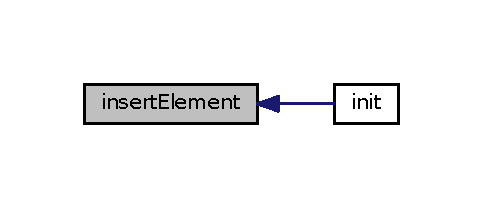
\includegraphics[width=232pt]{engine_8c_af2a455cb77697f2c6c4ad4fa0479d8ee_icgraph}
\end{center}
\end{figure}


\hypertarget{engine_8c_aaa9b56690bf5f53d7d72d2e76d7ff74d}{\index{engine.\-c@{engine.\-c}!metric\-Min@{metric\-Min}}
\index{metric\-Min@{metric\-Min}!engine.c@{engine.\-c}}
\subsubsection[{metric\-Min}]{\setlength{\rightskip}{0pt plus 5cm}int metric\-Min (
\begin{DoxyParamCaption}
\item[{int}]{x1, }
\item[{int}]{y1, }
\item[{int}]{x2, }
\item[{int}]{y2}
\end{DoxyParamCaption}
)}}\label{engine_8c_aaa9b56690bf5f53d7d72d2e76d7ff74d}


Finds lesser of two distances\-: between x or y coordinates. 


\begin{DoxyParams}[1]{Parametry}
\mbox{\tt in}  & {\em x1} & X coordinate of first point on board. \\
\hline
\mbox{\tt in}  & {\em y1} & Y coordinate of first point on board. \\
\hline
\mbox{\tt in}  & {\em x2} & X coordinate of second point on board. \\
\hline
\mbox{\tt in}  & {\em y2} & Y coordinate of second point on board.\\
\hline
\end{DoxyParams}
\begin{DoxyReturn}{Zwraca}
Minimum of $\vert$x1 -\/ x2$\vert$ and $\vert$y1 -\/ y2$\vert$. 
\end{DoxyReturn}


Oto graf wywołań dla tej funkcji\-:
\nopagebreak
\begin{figure}[H]
\begin{center}
\leavevmode
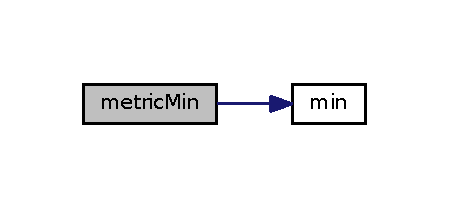
\includegraphics[width=216pt]{engine_8c_aaa9b56690bf5f53d7d72d2e76d7ff74d_cgraph}
\end{center}
\end{figure}


\hypertarget{engine_8c_abd8bbcfabb3ddef2ccaafb9928a37b95}{\index{engine.\-c@{engine.\-c}!min@{min}}
\index{min@{min}!engine.c@{engine.\-c}}
\subsubsection[{min}]{\setlength{\rightskip}{0pt plus 5cm}int min (
\begin{DoxyParamCaption}
\item[{int}]{a, }
\item[{int}]{b}
\end{DoxyParamCaption}
)}}\label{engine_8c_abd8bbcfabb3ddef2ccaafb9928a37b95}


Returns lesser value of two ints. 


\begin{DoxyParams}[1]{Parametry}
\mbox{\tt in}  & {\em a} & First value. \\
\hline
\mbox{\tt in}  & {\em b} & Second value.\\
\hline
\end{DoxyParams}
\begin{DoxyReturn}{Zwraca}
lesser value. 
\end{DoxyReturn}


Oto graf wywoływań tej funkcji\-:
\nopagebreak
\begin{figure}[H]
\begin{center}
\leavevmode
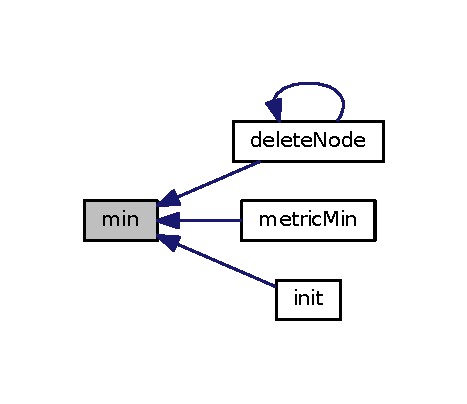
\includegraphics[width=224pt]{engine_8c_abd8bbcfabb3ddef2ccaafb9928a37b95_icgraph}
\end{center}
\end{figure}


\hypertarget{engine_8c_a17be2b87232c11cc093398d574452aa5}{\index{engine.\-c@{engine.\-c}!move@{move}}
\index{move@{move}!engine.c@{engine.\-c}}
\subsubsection[{move}]{\setlength{\rightskip}{0pt plus 5cm}int move (
\begin{DoxyParamCaption}
\item[{int}]{x1, }
\item[{int}]{y1, }
\item[{int}]{x2, }
\item[{int}]{y2, }
\item[{int}]{n, }
\item[{bool}]{my\-Turn, }
\item[{{\bf Tree\-Node} $\ast$$\ast$}]{tree, }
\item[{char $\ast$$\ast$}]{board, }
\item[{int}]{m, }
\item[{int}]{turns, }
\item[{int}]{my\-Number}
\end{DoxyParamCaption}
)}}\label{engine_8c_a17be2b87232c11cc093398d574452aa5}


Makes a move. 


\begin{DoxyParams}[1]{Parametry}
\mbox{\tt in}  & {\em x1} & Column number before a move. \\
\hline
\mbox{\tt in}  & {\em y1} & Row number before a move. \\
\hline
\mbox{\tt in}  & {\em x2} & Column number after a move. \\
\hline
\mbox{\tt in}  & {\em y2} & Row number before a move. \\
\hline
\mbox{\tt in}  & {\em n} & Size of a board. \\
\hline
\mbox{\tt in}  & {\em players1\-Turn} & Information if it is first player who moves a \hyperlink{structPiece}{Piece}. \\
\hline
\mbox{\tt in,out}  & {\em tree} & Tree containing nodes with all existing pieces. \\
\hline
\mbox{\tt in}  & {\em p1\-Initialized} & Information if I\-N\-I\-T of the first player has already been called. \\
\hline
\mbox{\tt in}  & {\em p2\-Initialized} & Information if I\-N\-I\-T of the second player has already been called. \\
\hline
\mbox{\tt in,out}  & {\em board} & Array representing top left part of a board. \\
\hline
\mbox{\tt in}  & {\em m} & Size of board. \\
\hline
\mbox{\tt in}  & {\em turns} & Number of remaining turns.\\
\hline
\end{DoxyParams}
\begin{DoxyReturn}{Zwraca}
C\-O\-N\-T\-I\-N\-U\-E if all arguments were correct. 

P1\-\_\-\-W\-I\-N if second player's king is beaten. 

P2\-\_\-\-W\-I\-N if first player's king is beaten. 

D\-R\-A\-W if both kings are beaten. 

I\-N\-P\-U\-T\-\_\-\-E\-R\-R\-O\-R if there was an input error. 
\end{DoxyReturn}


Oto graf wywołań dla tej funkcji\-:
\nopagebreak
\begin{figure}[H]
\begin{center}
\leavevmode
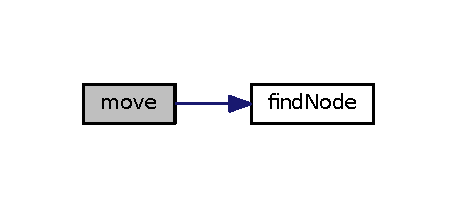
\includegraphics[width=220pt]{engine_8c_a17be2b87232c11cc093398d574452aa5_cgraph}
\end{center}
\end{figure}


\hypertarget{engine_8c_ab1554076e8bcda9021d6a6273c21af4c}{\index{engine.\-c@{engine.\-c}!print\-Topleft@{print\-Topleft}}
\index{print\-Topleft@{print\-Topleft}!engine.c@{engine.\-c}}
\subsubsection[{print\-Topleft}]{\setlength{\rightskip}{0pt plus 5cm}void print\-Topleft (
\begin{DoxyParamCaption}
\item[{char $\ast$$\ast$}]{board, }
\item[{int}]{m}
\end{DoxyParamCaption}
)}}\label{engine_8c_ab1554076e8bcda9021d6a6273c21af4c}


Prints (into stdout) top-\/left corner of the board of size m x m. 


\begin{DoxyParams}[1]{Parametry}
\mbox{\tt in}  & {\em board} & Array representing top left part of a board. \\
\hline
\mbox{\tt in}  & {\em m} & Size of board. \\
\hline
\end{DoxyParams}
\hypertarget{engine_8c_ac274a9b90ffa3c10e8c9ef7ae2ca98c6}{\index{engine.\-c@{engine.\-c}!produce\-Knight@{produce\-Knight}}
\index{produce\-Knight@{produce\-Knight}!engine.c@{engine.\-c}}
\subsubsection[{produce\-Knight}]{\setlength{\rightskip}{0pt plus 5cm}int produce\-Knight (
\begin{DoxyParamCaption}
\item[{int}]{x1, }
\item[{int}]{y1, }
\item[{int}]{x2, }
\item[{int}]{y2, }
\item[{int}]{n, }
\item[{bool}]{my\-Turn, }
\item[{int}]{my\-Number, }
\item[{{\bf Tree\-Node} $\ast$$\ast$}]{tree, }
\item[{char $\ast$$\ast$}]{board, }
\item[{int}]{m, }
\item[{int}]{turns}
\end{DoxyParamCaption}
)}}\label{engine_8c_ac274a9b90ffa3c10e8c9ef7ae2ca98c6}


Produces a knight. 

Knight can be produced only by a peasant who wasn't moved for 2 turns. Target field cannot be occupied.


\begin{DoxyParams}[1]{Parametry}
\mbox{\tt in}  & {\em x1} & Column number of a peasant. \\
\hline
\mbox{\tt in}  & {\em y1} & Row number of a peasant. \\
\hline
\mbox{\tt in}  & {\em x2} & Column number of a free field where peasant is to produce knight to. \\
\hline
\mbox{\tt in}  & {\em y2} & Row number of a free field where peasant is to produce knight to. \\
\hline
\mbox{\tt in,out}  & {\em tree} & Tree containing nodes with all existing pieces. \\
\hline
\mbox{\tt in}  & {\em p1\-Initialized} & Information if I\-N\-I\-T of the first player has already been called. \\
\hline
\mbox{\tt in}  & {\em p2\-Initialized} & Information if I\-N\-I\-T of the second player has already been called. \\
\hline
\mbox{\tt in,out}  & {\em board} & Array representing top left part of a board. \\
\hline
\mbox{\tt in}  & {\em m} & Size of board. \\
\hline
\mbox{\tt in}  & {\em turns} & Number of remaining turns.\\
\hline
\end{DoxyParams}
\begin{DoxyReturn}{Zwraca}
C\-O\-N\-T\-I\-N\-U\-E if all arguments were correct. 

I\-N\-P\-U\-T\-\_\-\-E\-R\-R\-O\-R if there was an input error. 
\end{DoxyReturn}
\hypertarget{engine_8c_a610df406fe7f88d89ded2c1854c7d3aa}{\index{engine.\-c@{engine.\-c}!produce\-Peasant@{produce\-Peasant}}
\index{produce\-Peasant@{produce\-Peasant}!engine.c@{engine.\-c}}
\subsubsection[{produce\-Peasant}]{\setlength{\rightskip}{0pt plus 5cm}int produce\-Peasant (
\begin{DoxyParamCaption}
\item[{int}]{x1, }
\item[{int}]{y1, }
\item[{int}]{x2, }
\item[{int}]{y2, }
\item[{int}]{n, }
\item[{bool}]{my\-Turn, }
\item[{int}]{my\-Number, }
\item[{{\bf Tree\-Node} $\ast$$\ast$}]{tree, }
\item[{char $\ast$$\ast$}]{board, }
\item[{int}]{m, }
\item[{int}]{turns}
\end{DoxyParamCaption}
)}}\label{engine_8c_a610df406fe7f88d89ded2c1854c7d3aa}


Produces a peasant. 

Peasant can be produced only by a peasant who wasn't moved for 2 turns. Target field cannot be occupied.


\begin{DoxyParams}[1]{Parametry}
\mbox{\tt in}  & {\em x1} & Column number of an existing peasant. \\
\hline
\mbox{\tt in}  & {\em y1} & Row number of an existing peasant. \\
\hline
\mbox{\tt in}  & {\em x2} & Column number of a free field where peasant is to produce a new peasant to. \\
\hline
\mbox{\tt in}  & {\em y2} & Row number of a free field where peasant is to produce a new peasant to. \\
\hline
\mbox{\tt in,out}  & {\em tree} & Tree containing nodes with all existing pieces. \\
\hline
\mbox{\tt in}  & {\em p1\-Initialized} & Information if I\-N\-I\-T of the first player has already been called. \\
\hline
\mbox{\tt in}  & {\em p2\-Initialized} & Information if I\-N\-I\-T of the second player has already been called. \\
\hline
\mbox{\tt in,out}  & {\em board} & Array representing top left part of a board. \\
\hline
\mbox{\tt in}  & {\em m} & Size of board. \\
\hline
\mbox{\tt in}  & {\em turns} & Number of remaining turns.\\
\hline
\end{DoxyParams}
\begin{DoxyReturn}{Zwraca}
C\-O\-N\-T\-I\-N\-U\-E if all arguments were correct. 

I\-N\-P\-U\-T\-\_\-\-E\-R\-R\-O\-R if there was an input error. 
\end{DoxyReturn}
\hypertarget{engine_8c_a0776cd662f5c945bb00f5950ab384fcf}{\index{engine.\-c@{engine.\-c}!start\-Game@{start\-Game}}
\index{start\-Game@{start\-Game}!engine.c@{engine.\-c}}
\subsubsection[{start\-Game}]{\setlength{\rightskip}{0pt plus 5cm}void start\-Game (
\begin{DoxyParamCaption}
\item[{{\bf Tree\-Node} $\ast$$\ast$}]{tree}
\end{DoxyParamCaption}
)}}\label{engine_8c_a0776cd662f5c945bb00f5950ab384fcf}


Initializes a game. 

Needed before first I\-N\-I\-T.


\begin{DoxyParams}[1]{Parametry}
\mbox{\tt in,out}  & {\em tree} & Tree containing nodes with all existing pieces. \\
\hline
\end{DoxyParams}

\hypertarget{engine_8h}{\section{Dokumentacja pliku engine.\-h}
\label{engine_8h}\index{engine.\-h@{engine.\-h}}
}


Interface of game engine.  


{\ttfamily \#include $<$stdbool.\-h$>$}\\*
Wykres zależności załączania dla engine.\-h\-:\nopagebreak
\begin{figure}[H]
\begin{center}
\leavevmode
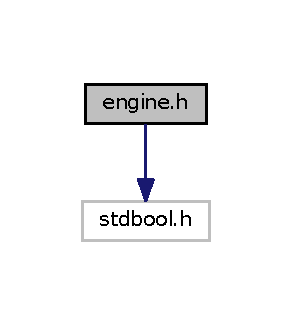
\includegraphics[width=140pt]{engine_8h__incl}
\end{center}
\end{figure}
Ten wykres pokazuje, które pliki bezpośrednio lub pośrednio załączają ten plik\-:\nopagebreak
\begin{figure}[H]
\begin{center}
\leavevmode
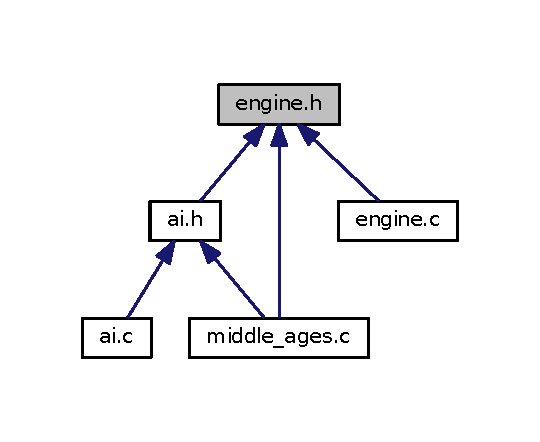
\includegraphics[width=166pt]{engine_8h__dep__incl}
\end{center}
\end{figure}
\subsection*{Struktury danych}
\begin{DoxyCompactItemize}
\item 
struct \hyperlink{structPiece}{Piece}
\begin{DoxyCompactList}\small\item\em Struct of \hyperlink{structPiece}{Piece}. \end{DoxyCompactList}\item 
struct \hyperlink{structTreeNode}{Tree\-Node}
\begin{DoxyCompactList}\small\item\em Struct of a tree containing pieces. \end{DoxyCompactList}\end{DoxyCompactItemize}
\subsection*{Definicje}
\begin{DoxyCompactItemize}
\item 
\hypertarget{engine_8h_ab711666ad09d7f6c0b91576525ea158e}{\#define {\bfseries C\-O\-N\-T\-I\-N\-U\-E}~0}\label{engine_8h_ab711666ad09d7f6c0b91576525ea158e}

\item 
\hypertarget{engine_8h_a288116f92845fddefeb044f5b84bc889}{\#define {\bfseries I\-N\-P\-U\-T\-\_\-\-E\-R\-R\-O\-R}~42}\label{engine_8h_a288116f92845fddefeb044f5b84bc889}

\item 
\hypertarget{engine_8h_a7a7cd353a6274e8c0dbb698113e7e194}{\#define {\bfseries D\-R\-A\-W}~1}\label{engine_8h_a7a7cd353a6274e8c0dbb698113e7e194}

\item 
\hypertarget{engine_8h_a2199bc4c776dbd7a4248aeef9e5dd8a1}{\#define {\bfseries D\-R\-A\-W\-\_\-\-A\-F\-T\-E\-R\-\_\-\-E\-N\-D\-\_\-\-T\-U\-R\-N}~5}\label{engine_8h_a2199bc4c776dbd7a4248aeef9e5dd8a1}

\item 
\hypertarget{engine_8h_a6ee3d6fa4e432d9456967fd82533de48}{\#define {\bfseries E\-N\-D\-\_\-\-T\-U\-R\-N}~2}\label{engine_8h_a6ee3d6fa4e432d9456967fd82533de48}

\item 
\hypertarget{engine_8h_a4db4e218f5d127d392593464377e7dbe}{\#define {\bfseries P1\-\_\-\-W\-I\-N}~3}\label{engine_8h_a4db4e218f5d127d392593464377e7dbe}

\item 
\hypertarget{engine_8h_a4081f92247bfc37403cab4610a4681a0}{\#define {\bfseries P2\-\_\-\-W\-I\-N}~4}\label{engine_8h_a4081f92247bfc37403cab4610a4681a0}

\end{DoxyCompactItemize}
\subsection*{Definicje typów}
\begin{DoxyCompactItemize}
\item 
typedef struct \hyperlink{structPiece}{Piece} \hyperlink{engine_8h_ad1ff76ab9261121f9492d0e79b03d586}{Piece}
\begin{DoxyCompactList}\small\item\em Struct of \hyperlink{structPiece}{Piece}. \end{DoxyCompactList}\item 
typedef struct \hyperlink{structTreeNode}{Tree\-Node} \hyperlink{engine_8h_a85a7513d1b1c40e8d6267a812ee61b9d}{Tree\-Node}
\begin{DoxyCompactList}\small\item\em Struct of a tree containing pieces. \end{DoxyCompactList}\end{DoxyCompactItemize}
\subsection*{Funkcje}
\begin{DoxyCompactItemize}
\item 
void \hyperlink{engine_8h_a0776cd662f5c945bb00f5950ab384fcf}{start\-Game} (\hyperlink{structTreeNode}{Tree\-Node} $\ast$$\ast$tree)
\begin{DoxyCompactList}\small\item\em Initializes a game. \end{DoxyCompactList}\item 
void \hyperlink{engine_8h_ac959cf8cbd90d8dc203659e8a8871664}{end\-Game} (\hyperlink{structTreeNode}{Tree\-Node} $\ast$$\ast$tree, int $\ast$result, char $\ast$$\ast$$\ast$board, int m)
\begin{DoxyCompactList}\small\item\em Frees memory. \end{DoxyCompactList}\item 
int \hyperlink{engine_8h_a4b24a63ab775b24fe4c652d06622f948}{init} (int n, int k, int p, int x1, int y1, int x2, int y2, \hyperlink{structTreeNode}{Tree\-Node} $\ast$$\ast$tree, int $\ast$n\-My, int $\ast$k\-My, bool $\ast$p1\-Initialized, bool $\ast$p2\-Initialized, char $\ast$$\ast$board, int $\ast$m)
\begin{DoxyCompactList}\small\item\em Initializes a game with size of a board, number of rounds and positions of kings. \end{DoxyCompactList}\item 
int \hyperlink{engine_8h_a823c9d0dc71ea5ea68cb1dafb42bce7a}{move} (int x1, int y1, int x2, int y2, int n, bool players1\-Turn, \hyperlink{structTreeNode}{Tree\-Node} $\ast$$\ast$tree, bool p1\-Initialized, bool p2\-Initialized, char $\ast$$\ast$board, int m, int turns)
\begin{DoxyCompactList}\small\item\em Makes a move. \end{DoxyCompactList}\item 
int \hyperlink{engine_8h_af5b7f337e6e7f58324ef24379f89d970}{produce\-Knight} (int x1, int y1, int x2, int y2, int n, bool players1\-Turn, \hyperlink{structTreeNode}{Tree\-Node} $\ast$$\ast$tree, bool p1\-Initialized, bool p2\-Initialized, char $\ast$$\ast$board, int m, int turns)
\begin{DoxyCompactList}\small\item\em Produces a knight. \end{DoxyCompactList}\item 
int \hyperlink{engine_8h_a82b7c406c0c1116d123ccccd06950a68}{produce\-Peasant} (int x1, int y1, int x2, int y2, int n, bool players1\-Turn, \hyperlink{structTreeNode}{Tree\-Node} $\ast$$\ast$tree, bool p1\-Initialized, bool p2\-Initialized, char $\ast$$\ast$board, int m, int turns)
\begin{DoxyCompactList}\small\item\em Produces a peasant. \end{DoxyCompactList}\item 
int \hyperlink{engine_8h_adff6ca550bc33a22dc1e6966c7a5d608}{end\-Turn} (int $\ast$turns, bool $\ast$players1\-Turn, \hyperlink{structTreeNode}{Tree\-Node} $\ast$$\ast$tree, bool p1\-Initialized, bool p2\-Initialized)
\begin{DoxyCompactList}\small\item\em Ends a turn. \end{DoxyCompactList}\item 
void \hyperlink{engine_8h_ab1554076e8bcda9021d6a6273c21af4c}{print\-Topleft} (char $\ast$$\ast$board, int m)
\begin{DoxyCompactList}\small\item\em Prints (into stdout) top-\/left corner of the board of size m x m. \end{DoxyCompactList}\item 
char $\ast$$\ast$ \hyperlink{engine_8h_a6e2f079a3de8efe3d5d507181cee3153}{allocate\-Memory} (int m)
\begin{DoxyCompactList}\small\item\em Allocates space for m by m array and fills it with dot. \end{DoxyCompactList}\item 
int \hyperlink{engine_8h_abd8bbcfabb3ddef2ccaafb9928a37b95}{min} (int a, int b)
\begin{DoxyCompactList}\small\item\em Returns lesser value of two ints. \end{DoxyCompactList}\end{DoxyCompactItemize}


\subsection{Opis szczegółowy}
Interface of game engine. Contains all functions needed to start, play, read input (and check parameters), print output and end the game. 

\subsection{Dokumentacja definicji typów}
\hypertarget{engine_8h_ad1ff76ab9261121f9492d0e79b03d586}{\index{engine.\-h@{engine.\-h}!Piece@{Piece}}
\index{Piece@{Piece}!engine.h@{engine.\-h}}
\subsubsection[{Piece}]{\setlength{\rightskip}{0pt plus 5cm}typedef struct {\bf Piece}  {\bf Piece}}}\label{engine_8h_ad1ff76ab9261121f9492d0e79b03d586}


Struct of \hyperlink{structPiece}{Piece}. 


\begin{DoxyParams}{Parametry}
{\em x} & Number of column of a piece. \\
\hline
{\em y} & Number of row of a piece. \\
\hline
{\em ch} & Char representing a piece('K', 'C', 'R', 'k', 'c' or 'r') \\
\hline
{\em turn\-Moved} & Last turn this piece was moved. \\
\hline
{\em moved} & True if the piece was moved last turn. \\
\hline
\end{DoxyParams}
\hypertarget{engine_8h_a85a7513d1b1c40e8d6267a812ee61b9d}{\index{engine.\-h@{engine.\-h}!Tree\-Node@{Tree\-Node}}
\index{Tree\-Node@{Tree\-Node}!engine.h@{engine.\-h}}
\subsubsection[{Tree\-Node}]{\setlength{\rightskip}{0pt plus 5cm}typedef struct {\bf Tree\-Node}  {\bf Tree\-Node}}}\label{engine_8h_a85a7513d1b1c40e8d6267a812ee61b9d}


Struct of a tree containing pieces. 


\begin{DoxyParams}{Parametry}
{\em \hyperlink{structPiece}{Piece}} & Struct containing parameters of a \hyperlink{structPiece}{Piece} \\
\hline
\end{DoxyParams}
\begin{DoxySeeAlso}{Zobacz również}
\hyperlink{structPiece}{Piece} 
\end{DoxySeeAlso}

\begin{DoxyParams}{Parametry}
{\em left} & Pointer to left son of the node. \\
\hline
{\em right} & Pointer to right son of the node. \\
\hline
\end{DoxyParams}


\subsection{Dokumentacja funkcji}
\hypertarget{engine_8h_a6e2f079a3de8efe3d5d507181cee3153}{\index{engine.\-h@{engine.\-h}!allocate\-Memory@{allocate\-Memory}}
\index{allocate\-Memory@{allocate\-Memory}!engine.h@{engine.\-h}}
\subsubsection[{allocate\-Memory}]{\setlength{\rightskip}{0pt plus 5cm}char$\ast$$\ast$ allocate\-Memory (
\begin{DoxyParamCaption}
\item[{int}]{m}
\end{DoxyParamCaption}
)}}\label{engine_8h_a6e2f079a3de8efe3d5d507181cee3153}


Allocates space for m by m array and fills it with dot. 


\begin{DoxyParams}[1]{Parametry}
\mbox{\tt in}  & {\em m} & Size of the array. \\
\hline
\end{DoxyParams}
\begin{DoxyReturn}{Zwraca}
allocated array 
\end{DoxyReturn}
\hypertarget{engine_8h_ac959cf8cbd90d8dc203659e8a8871664}{\index{engine.\-h@{engine.\-h}!end\-Game@{end\-Game}}
\index{end\-Game@{end\-Game}!engine.h@{engine.\-h}}
\subsubsection[{end\-Game}]{\setlength{\rightskip}{0pt plus 5cm}void end\-Game (
\begin{DoxyParamCaption}
\item[{{\bf Tree\-Node} $\ast$$\ast$}]{tree, }
\item[{int $\ast$}]{result, }
\item[{char $\ast$$\ast$$\ast$}]{board, }
\item[{int}]{m}
\end{DoxyParamCaption}
)}}\label{engine_8h_ac959cf8cbd90d8dc203659e8a8871664}


Frees memory. 

Needed after finishing game. 
\begin{DoxyParams}[1]{Parametry}
\mbox{\tt in,out}  & {\em tree} & Tree containing nodes with all existing pieces. \\
\hline
\mbox{\tt out}  & {\em result} & Variable keeping result of the game so that proper output can be printed. Also changed to 0 or 42 and returned in main function. \\
\hline
\mbox{\tt in,out}  & {\em board} & Array representing top left part of a board. \\
\hline
\mbox{\tt in}  & {\em m} & Size of board. \\
\hline
\end{DoxyParams}
\hypertarget{engine_8h_adff6ca550bc33a22dc1e6966c7a5d608}{\index{engine.\-h@{engine.\-h}!end\-Turn@{end\-Turn}}
\index{end\-Turn@{end\-Turn}!engine.h@{engine.\-h}}
\subsubsection[{end\-Turn}]{\setlength{\rightskip}{0pt plus 5cm}int end\-Turn (
\begin{DoxyParamCaption}
\item[{int $\ast$}]{turns, }
\item[{bool $\ast$}]{players1\-Turn, }
\item[{{\bf Tree\-Node} $\ast$$\ast$}]{tree, }
\item[{bool}]{p1\-Initialized, }
\item[{bool}]{p2\-Initialized}
\end{DoxyParamCaption}
)}}\label{engine_8h_adff6ca550bc33a22dc1e6966c7a5d608}


Ends a turn. 

Changes current player. Checks if both players ended their turns, then \char`\"{}refreshes\char`\"{} all pieces before next turn and changes and decreases remaining number of turns. 
\begin{DoxyParams}[1]{Parametry}
\mbox{\tt in,out}  & {\em turns} & Number of remaining turns. \\
\hline
\mbox{\tt in,out}  & {\em players1\-Turn} & Informs if turn being ended was player 1's. \\
\hline
\mbox{\tt in,out}  & {\em tree} & Tree containing nodes with all existing pieces. \\
\hline
\mbox{\tt in}  & {\em p1\-Initialized} & Information if I\-N\-I\-T of the first player has already been called. \\
\hline
\mbox{\tt in}  & {\em p2\-Initialized} & Information if I\-N\-I\-T of the second player has already been called. \\
\hline
\end{DoxyParams}
\hypertarget{engine_8h_a4b24a63ab775b24fe4c652d06622f948}{\index{engine.\-h@{engine.\-h}!init@{init}}
\index{init@{init}!engine.h@{engine.\-h}}
\subsubsection[{init}]{\setlength{\rightskip}{0pt plus 5cm}int init (
\begin{DoxyParamCaption}
\item[{int}]{n, }
\item[{int}]{k, }
\item[{int}]{p, }
\item[{int}]{x1, }
\item[{int}]{y1, }
\item[{int}]{x2, }
\item[{int}]{y2, }
\item[{{\bf Tree\-Node} $\ast$$\ast$}]{tree, }
\item[{int $\ast$}]{n\-My, }
\item[{int $\ast$}]{k\-My, }
\item[{bool $\ast$}]{p1\-Initialized, }
\item[{bool $\ast$}]{p2\-Initialized, }
\item[{char $\ast$$\ast$}]{board, }
\item[{int $\ast$}]{m}
\end{DoxyParamCaption}
)}}\label{engine_8h_a4b24a63ab775b24fe4c652d06622f948}


Initializes a game with size of a board, number of rounds and positions of kings. 

One I\-N\-I\-T for each player is needed before any other \hyperlink{structCommand}{Command}. 
\begin{DoxyParams}[1]{Parametry}
\mbox{\tt in}  & {\em n} & Size of a board. \\
\hline
\mbox{\tt in}  & {\em k} & Number of turns of each player. \\
\hline
\mbox{\tt in}  & {\em p} & Number of player for whom initialization is called. \\
\hline
\mbox{\tt in}  & {\em x1} & Column number of first player's king. \\
\hline
\mbox{\tt in}  & {\em y1} & Row number of first player's king. \\
\hline
\mbox{\tt in}  & {\em x2} & Column number of second player's king. \\
\hline
\mbox{\tt in}  & {\em y2} & Row number of second player's king. \\
\hline
\mbox{\tt in,out}  & {\em tree} & Tree containing nodes with all existing pieces. \\
\hline
\mbox{\tt out}  & {\em n\-My} & Variable keeping the size of board. \\
\hline
\mbox{\tt out}  & {\em k\-My} & Variable keeping number of turns. \\
\hline
\mbox{\tt in}  & {\em p1\-Initialized} & Information if I\-N\-I\-T of the first player has already been called. \\
\hline
\mbox{\tt in}  & {\em p2\-Initialized} & Information if I\-N\-I\-T of the second player has already been called. \\
\hline
\mbox{\tt in,out}  & {\em board} & Array representing top left part of a board. \\
\hline
\mbox{\tt in}  & {\em m} & Size of board. \\
\hline
\end{DoxyParams}
\begin{DoxyReturn}{Zwraca}
C\-O\-N\-T\-I\-N\-U\-E if all arguments were correct. 

I\-N\-P\-U\-T\-\_\-\-E\-R\-R\-O\-R if there was an input error. 
\end{DoxyReturn}


Oto graf wywołań dla tej funkcji\-:\nopagebreak
\begin{figure}[H]
\begin{center}
\leavevmode
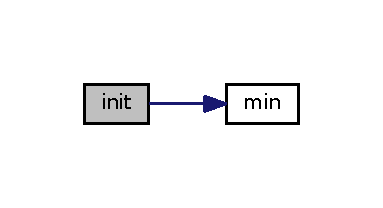
\includegraphics[width=184pt]{engine_8h_a4b24a63ab775b24fe4c652d06622f948_cgraph}
\end{center}
\end{figure}


\hypertarget{engine_8h_abd8bbcfabb3ddef2ccaafb9928a37b95}{\index{engine.\-h@{engine.\-h}!min@{min}}
\index{min@{min}!engine.h@{engine.\-h}}
\subsubsection[{min}]{\setlength{\rightskip}{0pt plus 5cm}int min (
\begin{DoxyParamCaption}
\item[{int}]{a, }
\item[{int}]{b}
\end{DoxyParamCaption}
)}}\label{engine_8h_abd8bbcfabb3ddef2ccaafb9928a37b95}


Returns lesser value of two ints. 


\begin{DoxyParams}[1]{Parametry}
\mbox{\tt in}  & {\em a} & First value. \\
\hline
\mbox{\tt in}  & {\em b} & Second value. \\
\hline
\end{DoxyParams}
\begin{DoxyReturn}{Zwraca}
lesser value. 
\end{DoxyReturn}


Oto graf wywoływań tej funkcji\-:\nopagebreak
\begin{figure}[H]
\begin{center}
\leavevmode
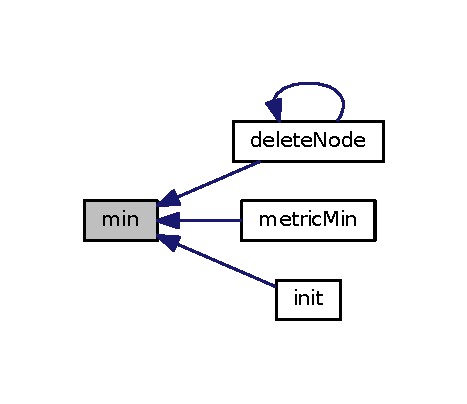
\includegraphics[width=184pt]{engine_8h_abd8bbcfabb3ddef2ccaafb9928a37b95_icgraph}
\end{center}
\end{figure}


\hypertarget{engine_8h_a823c9d0dc71ea5ea68cb1dafb42bce7a}{\index{engine.\-h@{engine.\-h}!move@{move}}
\index{move@{move}!engine.h@{engine.\-h}}
\subsubsection[{move}]{\setlength{\rightskip}{0pt plus 5cm}int move (
\begin{DoxyParamCaption}
\item[{int}]{x1, }
\item[{int}]{y1, }
\item[{int}]{x2, }
\item[{int}]{y2, }
\item[{int}]{n, }
\item[{bool}]{players1\-Turn, }
\item[{{\bf Tree\-Node} $\ast$$\ast$}]{tree, }
\item[{bool}]{p1\-Initialized, }
\item[{bool}]{p2\-Initialized, }
\item[{char $\ast$$\ast$}]{board, }
\item[{int}]{m, }
\item[{int}]{turns}
\end{DoxyParamCaption}
)}}\label{engine_8h_a823c9d0dc71ea5ea68cb1dafb42bce7a}


Makes a move. 


\begin{DoxyParams}[1]{Parametry}
\mbox{\tt in}  & {\em x1} & Column number before a move. \\
\hline
\mbox{\tt in}  & {\em y1} & Row number before a move. \\
\hline
\mbox{\tt in}  & {\em x2} & Column number after a move. \\
\hline
\mbox{\tt in}  & {\em y2} & Row number before a move. \\
\hline
\mbox{\tt in}  & {\em n} & Size of a board. \\
\hline
\mbox{\tt in}  & {\em players1\-Turn} & Information if it is first player who moves a \hyperlink{structPiece}{Piece}. \\
\hline
\mbox{\tt in,out}  & {\em tree} & Tree containing nodes with all existing pieces. \\
\hline
\mbox{\tt in}  & {\em p1\-Initialized} & Information if I\-N\-I\-T of the first player has already been called. \\
\hline
\mbox{\tt in}  & {\em p2\-Initialized} & Information if I\-N\-I\-T of the second player has already been called. \\
\hline
\mbox{\tt in,out}  & {\em board} & Array representing top left part of a board. \\
\hline
\mbox{\tt in}  & {\em m} & Size of board. \\
\hline
\mbox{\tt in}  & {\em turns} & Number of remaining turns. \\
\hline
\end{DoxyParams}
\begin{DoxyReturn}{Zwraca}
C\-O\-N\-T\-I\-N\-U\-E if all arguments were correct. 

P1\-\_\-\-W\-I\-N if second player's king is beaten. 

P2\-\_\-\-W\-I\-N if first player's king is beaten. 

D\-R\-A\-W if both kings are beaten. 

I\-N\-P\-U\-T\-\_\-\-E\-R\-R\-O\-R if there was an input error. 
\end{DoxyReturn}
\hypertarget{engine_8h_ab1554076e8bcda9021d6a6273c21af4c}{\index{engine.\-h@{engine.\-h}!print\-Topleft@{print\-Topleft}}
\index{print\-Topleft@{print\-Topleft}!engine.h@{engine.\-h}}
\subsubsection[{print\-Topleft}]{\setlength{\rightskip}{0pt plus 5cm}void print\-Topleft (
\begin{DoxyParamCaption}
\item[{char $\ast$$\ast$}]{board, }
\item[{int}]{m}
\end{DoxyParamCaption}
)}}\label{engine_8h_ab1554076e8bcda9021d6a6273c21af4c}


Prints (into stdout) top-\/left corner of the board of size m x m. 


\begin{DoxyParams}[1]{Parametry}
\mbox{\tt in}  & {\em board} & Array representing top left part of a board. \\
\hline
\mbox{\tt in}  & {\em m} & Size of board. \\
\hline
\end{DoxyParams}
\hypertarget{engine_8h_af5b7f337e6e7f58324ef24379f89d970}{\index{engine.\-h@{engine.\-h}!produce\-Knight@{produce\-Knight}}
\index{produce\-Knight@{produce\-Knight}!engine.h@{engine.\-h}}
\subsubsection[{produce\-Knight}]{\setlength{\rightskip}{0pt plus 5cm}int produce\-Knight (
\begin{DoxyParamCaption}
\item[{int}]{x1, }
\item[{int}]{y1, }
\item[{int}]{x2, }
\item[{int}]{y2, }
\item[{int}]{n, }
\item[{bool}]{players1\-Turn, }
\item[{{\bf Tree\-Node} $\ast$$\ast$}]{tree, }
\item[{bool}]{p1\-Initialized, }
\item[{bool}]{p2\-Initialized, }
\item[{char $\ast$$\ast$}]{board, }
\item[{int}]{m, }
\item[{int}]{turns}
\end{DoxyParamCaption}
)}}\label{engine_8h_af5b7f337e6e7f58324ef24379f89d970}


Produces a knight. 

Knight can be produced only by a peasant who wasn't moved for 2 turns. Target field cannot be occupied. 
\begin{DoxyParams}[1]{Parametry}
\mbox{\tt in}  & {\em x1} & Column number of a peasant. \\
\hline
\mbox{\tt in}  & {\em y1} & Row number of a peasant. \\
\hline
\mbox{\tt in}  & {\em x2} & Column number of a free field where peasant is to produce knight to. \\
\hline
\mbox{\tt in}  & {\em y2} & Row number of a free field where peasant is to produce knight to. \\
\hline
\mbox{\tt in,out}  & {\em tree} & Tree containing nodes with all existing pieces. \\
\hline
\mbox{\tt in}  & {\em p1\-Initialized} & Information if I\-N\-I\-T of the first player has already been called. \\
\hline
\mbox{\tt in}  & {\em p2\-Initialized} & Information if I\-N\-I\-T of the second player has already been called. \\
\hline
\mbox{\tt in,out}  & {\em board} & Array representing top left part of a board. \\
\hline
\mbox{\tt in}  & {\em m} & Size of board. \\
\hline
\mbox{\tt in}  & {\em turns} & Number of remaining turns. \\
\hline
\end{DoxyParams}
\begin{DoxyReturn}{Zwraca}
C\-O\-N\-T\-I\-N\-U\-E if all arguments were correct. 

I\-N\-P\-U\-T\-\_\-\-E\-R\-R\-O\-R if there was an input error. 
\end{DoxyReturn}
\hypertarget{engine_8h_a82b7c406c0c1116d123ccccd06950a68}{\index{engine.\-h@{engine.\-h}!produce\-Peasant@{produce\-Peasant}}
\index{produce\-Peasant@{produce\-Peasant}!engine.h@{engine.\-h}}
\subsubsection[{produce\-Peasant}]{\setlength{\rightskip}{0pt plus 5cm}int produce\-Peasant (
\begin{DoxyParamCaption}
\item[{int}]{x1, }
\item[{int}]{y1, }
\item[{int}]{x2, }
\item[{int}]{y2, }
\item[{int}]{n, }
\item[{bool}]{players1\-Turn, }
\item[{{\bf Tree\-Node} $\ast$$\ast$}]{tree, }
\item[{bool}]{p1\-Initialized, }
\item[{bool}]{p2\-Initialized, }
\item[{char $\ast$$\ast$}]{board, }
\item[{int}]{m, }
\item[{int}]{turns}
\end{DoxyParamCaption}
)}}\label{engine_8h_a82b7c406c0c1116d123ccccd06950a68}


Produces a peasant. 

Peasant can be produced only by a peasant who wasn't moved for 2 turns. Target field cannot be occupied. 
\begin{DoxyParams}[1]{Parametry}
\mbox{\tt in}  & {\em x1} & Column number of an existing peasant. \\
\hline
\mbox{\tt in}  & {\em y1} & Row number of an existing peasant. \\
\hline
\mbox{\tt in}  & {\em x2} & Column number of a free field where peasant is to produce a new peasant to. \\
\hline
\mbox{\tt in}  & {\em y2} & Row number of a free field where peasant is to produce a new peasant to. \\
\hline
\mbox{\tt in,out}  & {\em tree} & Tree containing nodes with all existing pieces. \\
\hline
\mbox{\tt in}  & {\em p1\-Initialized} & Information if I\-N\-I\-T of the first player has already been called. \\
\hline
\mbox{\tt in}  & {\em p2\-Initialized} & Information if I\-N\-I\-T of the second player has already been called. \\
\hline
\mbox{\tt in,out}  & {\em board} & Array representing top left part of a board. \\
\hline
\mbox{\tt in}  & {\em m} & Size of board. \\
\hline
\mbox{\tt in}  & {\em turns} & Number of remaining turns. \\
\hline
\end{DoxyParams}
\begin{DoxyReturn}{Zwraca}
C\-O\-N\-T\-I\-N\-U\-E if all arguments were correct. 

I\-N\-P\-U\-T\-\_\-\-E\-R\-R\-O\-R if there was an input error. 
\end{DoxyReturn}
\hypertarget{engine_8h_a0776cd662f5c945bb00f5950ab384fcf}{\index{engine.\-h@{engine.\-h}!start\-Game@{start\-Game}}
\index{start\-Game@{start\-Game}!engine.h@{engine.\-h}}
\subsubsection[{start\-Game}]{\setlength{\rightskip}{0pt plus 5cm}void start\-Game (
\begin{DoxyParamCaption}
\item[{{\bf Tree\-Node} $\ast$$\ast$}]{tree}
\end{DoxyParamCaption}
)}}\label{engine_8h_a0776cd662f5c945bb00f5950ab384fcf}


Initializes a game. 

Needed before first I\-N\-I\-T. 
\begin{DoxyParams}[1]{Parametry}
\mbox{\tt in,out}  & {\em tree} & Tree containing nodes with all existing pieces. \\
\hline
\end{DoxyParams}

\hypertarget{middle__ages_8c}{\section{Dokumentacja pliku middle\-\_\-ages.\-c}
\label{middle__ages_8c}\index{middle\-\_\-ages.\-c@{middle\-\_\-ages.\-c}}
}


Main funtion of a game.  


{\ttfamily \#include $<$stdio.\-h$>$}\\*
{\ttfamily \#include $<$string.\-h$>$}\\*
{\ttfamily \#include $<$stdlib.\-h$>$}\\*
{\ttfamily \#include \char`\"{}parse.\-h\char`\"{}}\\*
{\ttfamily \#include \char`\"{}engine.\-h\char`\"{}}\\*
Wykres zależności załączania dla middle\-\_\-ages.\-c\-:\nopagebreak
\begin{figure}[H]
\begin{center}
\leavevmode
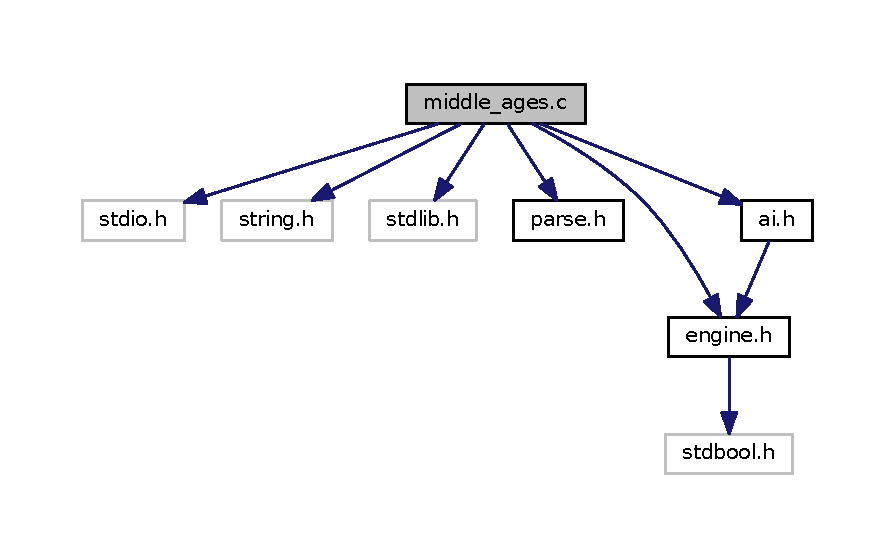
\includegraphics[width=350pt]{middle__ages_8c__incl}
\end{center}
\end{figure}
\subsection*{Funkcje}
\begin{DoxyCompactItemize}
\item 
\hypertarget{middle__ages_8c_ae66f6b31b5ad750f1fe042a706a4e3d4}{int {\bfseries main} ()}\label{middle__ages_8c_ae66f6b31b5ad750f1fe042a706a4e3d4}

\end{DoxyCompactItemize}


\subsection{Opis szczegółowy}
Main funtion of a game. Includes \hyperlink{parse_8h}{parse.\-h} to parse commands and \hyperlink{engine_8h}{engine.\-h} to perform all necessary commands as well as recognise correct input. \begin{DoxyReturn}{Zwraca}
0 if game ends properly(win or draw), or 42 if there was an input error. 
\end{DoxyReturn}

\hypertarget{parse_8h}{\section{Dokumentacja pliku parse.\-h}
\label{parse_8h}\index{parse.\-h@{parse.\-h}}
}


Interface of parser.  


Ten wykres pokazuje, które pliki bezpośrednio lub pośrednio załączają ten plik\-:\nopagebreak
\begin{figure}[H]
\begin{center}
\leavevmode
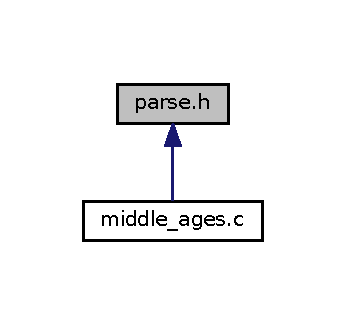
\includegraphics[width=166pt]{parse_8h__dep__incl}
\end{center}
\end{figure}
\subsection*{Struktury danych}
\begin{DoxyCompactItemize}
\item 
struct \hyperlink{structCommand}{Command}
\begin{DoxyCompactList}\small\item\em Struct of a \hyperlink{structCommand}{Command}. \end{DoxyCompactList}\end{DoxyCompactItemize}
\subsection*{Definicje typów}
\begin{DoxyCompactItemize}
\item 
typedef struct \hyperlink{structCommand}{Command} \hyperlink{parse_8h_a1e070cd9ac686a0bb549183eaf77290e}{Command}
\begin{DoxyCompactList}\small\item\em Struct of a \hyperlink{structCommand}{Command}. \end{DoxyCompactList}\end{DoxyCompactItemize}
\subsection*{Funkcje}
\begin{DoxyCompactItemize}
\item 
\hyperlink{structCommand}{Command} $\ast$ \hyperlink{parse_8h_a74bb0ea1e7abe5fa86309d56646b2e48}{parse\-Command} ()
\begin{DoxyCompactList}\small\item\em Reads a \hyperlink{structCommand}{Command}. \end{DoxyCompactList}\end{DoxyCompactItemize}


\subsection{Opis szczegółowy}
Interface of parser. Contains all functions needed to parse \hyperlink{structCommand}{Command} from input. 

\subsection{Dokumentacja definicji typów}
\hypertarget{parse_8h_a1e070cd9ac686a0bb549183eaf77290e}{\index{parse.\-h@{parse.\-h}!Command@{Command}}
\index{Command@{Command}!parse.h@{parse.\-h}}
\subsubsection[{Command}]{\setlength{\rightskip}{0pt plus 5cm}typedef struct {\bf Command}  {\bf Command}}}\label{parse_8h_a1e070cd9ac686a0bb549183eaf77290e}


Struct of a \hyperlink{structCommand}{Command}. 


\begin{DoxyParams}{Parametry}
{\em name} & Name of a \hyperlink{structCommand}{Command} or \char`\"{}\-E\-R\-R\-O\-R\char`\"{} if unexpected name was parsed. \\
\hline
{\em data\mbox{[}$\,$\mbox{]}} & Necessary arguments for each \hyperlink{structCommand}{Command} \\
\hline
\end{DoxyParams}


\subsection{Dokumentacja funkcji}
\hypertarget{parse_8h_a74bb0ea1e7abe5fa86309d56646b2e48}{\index{parse.\-h@{parse.\-h}!parse\-Command@{parse\-Command}}
\index{parse\-Command@{parse\-Command}!parse.h@{parse.\-h}}
\subsubsection[{parse\-Command}]{\setlength{\rightskip}{0pt plus 5cm}{\bf Command}$\ast$ parse\-Command (
\begin{DoxyParamCaption}
{}
\end{DoxyParamCaption}
)}}\label{parse_8h_a74bb0ea1e7abe5fa86309d56646b2e48}


Reads a \hyperlink{structCommand}{Command}. 

Returns \hyperlink{structCommand}{Command} with data points using '\hyperlink{structCommand}{Command}' structure. 
%--- End generated contents ---

% Index
\newpage
\phantomsection
\addcontentsline{toc}{chapter}{Indeks}
\printindex

\end{document}
